\documentclass{report}
\usepackage{arev}
\usepackage[T1]{fontenc}
\usepackage[a4paper, left=2.5cm, right= 2.5cm, top=2.5cm, bottom= 2.5cm]{geometry} %cambiar los márgenes
\usepackage{amsmath, amssymb, cancel, extarrows, amsthm }%símbolos matemáticos
\usepackage{wasysym}  %la carita triste
\usepackage{derivative}
\usepackage{physics}
\usepackage{graphicx, wrapfig}% Include figure files
\usepackage{subfig}
\usepackage{dcolumn}% Align table columns on decimal point
\usepackage{bm}% bold math
\usepackage{hyperref}% add hypertext capabilities
\usepackage{units}
\usepackage[spanish, es-tabla]{babel} %traducción al español
\usepackage{fancyhdr, ragged2e}
\setlength{\headheight}{13.07002pt}
\renewcommand{\footrulewidth}{0.4pt}
\usepackage{float}
\usepackage[symbol]{footmisc}
\usepackage{booktabs}
\usepackage{multirow}
\usepackage{multicol}
\usepackage[table,xcdraw]{xcolor}
\usepackage{xcolor, colortbl}
\usepackage{pagecolor}
\usepackage{tcolorbox}
\renewcommand{\thempfootnote}{\fnsymbol{mpfootnote}}
\newtcolorbox{mybox}{colback=gray!5!white,colframe=black!75!black}
\definecolor{cadetblue4}{rgb}{.33,.53,.55}
\definecolor{azulcrepuscular}{rgb}{.49,.62,.75}
\definecolor {atomictangerine} {rgb} {1.0, 0.6, 0.4}
\usepackage{longtable}
\usepackage{hyperref}
\hypersetup{
    colorlinks=true,
    linkcolor=black,
    filecolor=magenta,      
    urlcolor=blue,
    pdftitle={Apuntes de Geometría Diferencial \& Cálculo Tensorial},
    pdfpagemode=FullScreen,
    }

\renewcommand\familydefault{\sfdefault}
\addto\captionsspanish{
  \renewcommand{\contentsname}%
    {Índice de contenidos}%
}

\begin{document}
\newpagecolor{portada}
\begin{titlepage}
   \raggedright
       \vspace*{1cm}
       \textcolor{white}{\rule{\textwidth}{2pt}}
        \HUGE
       {\rmfamily \textbf{\textcolor{white}{Electrodinámica Clásica}}}
       
        \Large
       \vspace{0.5cm}
       {\rmfamily \textbf{\textcolor{white}{Manuel Lozano Bermúdez}}}

       \large
       \vspace{0.5 cm}
       {\rmfamily \textbf{\textcolor{white}{Curso 2023-2024, grupo C}}}
       \textcolor{white}{\rule{\textwidth}{2pt}}
        \vspace{1.5 cm}
       \begin{figure}[h]
           \centering
           \includegraphics[scale=.4]{FOTOS/portada.jpg}
           \label{fig:portada}
       \end{figure}

        \vspace*{\fill}
        
         \Large
         {\rmfamily \textcolor{white}{Comenzado el: 6 de septiembre de 2023}\\}
         {\rmfamily \textcolor{white}{Terminado el: 25 de septiembre de 2023 (SIN ACABAR)}}


\end{titlepage}
\restorepagecolor

\pagestyle{fancy}
\fancyhead[R]{}
\fancyfoot[L]{Manuel Lozano B.}
\fancyfoot[R]{GD$\&$CT}

\section*{Agradecimientos}

A Marcos, por revisar los apuntes, limpiarlos de erratas y por obligarme a mantener frescos mis conocimientos de la  asignatura. 

\tableofcontents

\part{Teoría}

\chapter{El espacio euclídeo $\mathbb{R}^n$. Teoría de curvas}
\section{Definición}
\large
El espacio vectorial $\mathbb{R}^n$ está formado por vectores de la forma:
$$
\mathbb{R}^n=\left \{ \mathbf{x}=(x_1,x_2,...,x_n);x_1,...,x_n\in \mathbb{R}\right \}
$$

Estos satisfacen las propiedades de espacio vectorial con respecto a las operaciones de producto interno y externo: $\mathbf{x+y},\lambda \mathbf{x}$ con $\lambda \in \mathbb{R}$.\\

La \emph{base canónica} de $\mathbb{R}^n$ es:
$$
\mathbf{e_1}=(1,0,...,0) \ , \ \mathbf{e_2}=(0,1,0,...,0) \ , \ ... \ , \ \mathbf{e_n}=(0,0,...,0,1)
$$

En la base canónica, cualquier vector genérico $\mathbf{x}\in \mathbb{R}^n$ se escribe como:
$$
\mathbf{x}=x_1\mathbf{e_1}+x_2\mathbf{e_2}+...+x_n\mathbf{e_n}=\sum_{i=1}^n x_i \mathbf{e_i}
$$

Además, si $\mathbf{x,y} \in \mathbb{R}^n$, definimos su \emph{producto escalar} como: 
$$
\mathbf{x\cdot y}=x_1y_1+x_2y_2+...+x_ny_n=\sum_{i=1}^n x_iy_i
$$
y la norma euclídea de un vector.
$$
||\mathbf{x}||=\sqrt{\mathbf{x\cdot x}}=\sqrt{\sum_{i=1}^n x_ix_i}
$$

Por tanto, la distancia entre dos puntos de $\mathbb{R}^n$ puede definirse como:

$$
d(\mathbf{x,y})=||\mathbf{x}-\mathbf{y}||=\sqrt{\sum_{i=1}^n(x_i-y_i)^2}
$$
%%%%AÑADIR GRÁFICO%%%%%
y el ángulo $\theta$ formado entre dos vectores $\mathbf{x}$ e $\mathbf{y}$ se define como:
$$
\cos{\theta}=\frac{\mathbf{x\cdot y}}{||\mathbf{x}||\cdot||\mathbf{y}||}
$$

Por lo tanto, la base canónica cumple que:
$$
\boxed{\mathbf{e_i\cdot e_j}=\delta_{ij}} \ , \ \delta_{ij}=\{ 1 \text{ si } i=j,\ 0 \text{ si } i\neq j\}
$$

Cualquier base que cumpla esa propiedad será una \emph{base ortonormal}. \\

Por otro lado, los vectores de una base se escriben de forma ordenada, lo que lleva al concepto de \emph{orientación} de una base. Dadas las bases de $\mathbb{R}^n\ ,B=\{ \mathbf{e_1},...,\mathbf{e_n}\}$ y $\tilde{B}=\{ \tilde{\mathbf{e_1}},...,\tilde{\mathbf{e_n}}\}$, diremos que tienen la misma orientación si el \emph{determinante de la matriz de cambio de base} es positivo.\\

\begin{mybox}
\begin{center}
Dados los vectores de $\tilde{B}$ en la base $B$:
$\tilde{\mathbf{e_i}}=\sum_{j=1}^nc_{ij}\mathbf{e_j}$\ ,\\
$B$ y $\tilde{B}$ tienen la \textbf{misma orientación} si $\det(C)>0$ \\
\noindent\rule{\textwidth}{0.5pt}
\end{center}
\underline{Ejemplo A:}
$\mathbb{R}^3$. Las bases:
$$
B=\{\mathbf{i,j,k}\} \ , \ \tilde{B}=\{ \mathbf{k,i,j}\} \quad \text{(permutación cíclica)}
$$ tienen la misma orientación.
Sin embargo, esto no se cumple con la base $\tilde{B}=\{ \mathbf{i,k,j}\}$. Las bases con idéntica orientación pueden transformarse entre ellas con un movimiento rígido (una rotación).
%%%%%AÑADIR DIBUJO%%%%%%%
\end{mybox}
\subsection{Producto vectorial y producto mixto}

En $\mathbb{R}^3$, se define el \emph{producto vectorial} de $\mathbf{x,y}\in \mathbb{R}^3$ como:
$$
\mathbf{x} \wedge \mathbf{y}=(x_2y_3-x_3y_2)\mathbf{i}+(x_3y_1-x_1y_3)\mathbf{j}+(x_1y_2-x_2y_1)\mathbf{k}
$$
donde $\{ \mathbf{i,j,k}\}$ es la base canónica de $\mathbb{R}^3$.\\

\textbf{Propiedades:}
\begin{enumerate}
    \item $||\mathbf{x} \wedge \mathbf{y}||=||\mathbf{x}||\cdot ||\mathbf{y}|| \sin{\theta}$. \\
    El módulo de $\mathbf{x} \wedge \mathbf{y}$ es el área del paralelogramo determinado por $\mathbf{x}$ e $\mathbf{y}$. \\
    %%%%%AÑADIR DIBUJO %%%%%%%

    \item $\mathbf{x} \parallel \mathbf{y} \implies \mathbf{x}\wedge \mathbf{y}=0$\\

    \item $\mathbf{x}\wedge \mathbf{y}=-\mathbf{y}\wedge \mathbf{x}$\\
\end{enumerate}

Se define el \emph{producto mixto} de $\mathbf{x,y,z}$ como:
$$
\mathbf{x \cdot }(\mathbf{y}\wedge \mathbf{z})=\left |
\begin{array}{ccc}
    x_1 &x_2 &x_3  \\
    y_1 &y_2 &y_3  \\
    z_1 &z_2 &z_3  \\
\end{array}
\right |=|\mathbf{x \quad y \quad z}|
$$\\

Geométricamente, el producto mixto se corresponde con el volumen del paralepípedo con lados $\mathbf{x,y,z}$.

\subsection{Isometrías en $\mathbb{R}^3$}
Una isometría de $\mathbb{R}^3$ es una transformación (aplicación) que \emph{preserva las distancias},
\begin{mybox}
    $T:\mathbb{R}^3 \rightarrow \mathbb{R}^3$.
    Si $T$ es una isometría, la distancia entre dos puntos del espacio se mantiene:
    $$
    d(\mathbf{x,y})=d(T\mathbf{x},T\mathbf{y})
    $$
\end{mybox}

Las isometrías en $\mathbb{R}^3$ (aunque se cumple en general en $\mathbb{R}^n$) son las \emph{traslaciones}, las \emph{rotaciones} y las \emph{reflexiones}.\\

%%%%%%AÑADIR DIBUJO%%%%%

El conjunto de isometrías de $\mathbb{R}^3$ (y de $\mathbb{R}^n$) forman un \emph{grupo}, conocido como \emph{grupo de isometrías}. Las isometrías se pueden escribir como:
\begin{align*}
    \boxed{T\mathbf{x}=R\mathbf{x}+\mathbf{b}} \quad , \qquad
    &\mathbf{b}\in \mathbb{R}^3\ , \ \mathbf{b}\equiv \text{const.}  \\
    &RR^t=\mathbb{I} \ , \ \text{(R es una matriz ortogonal)}
\end{align*}

Como consecuencia de esta propiedad, 
\begin{align*}
   &(R\mathbf{x},R\mathbf{y})=(R\mathbf{x})\cdot (R\mathbf{y})=\mathbf{x\cdot y}\\
    \implies &R\text{ conserva el producto escalar.} 
\end{align*}

Se cumple que $R$ transforma bases ortonromales en ortonormales.\\

Si $\mathbf{b}=\mathbf{0}$, tendremos el grupo de isometrías formado por las transformaciones ortogonales, $O(n)$ (en $\mathbb{R}^3$, $O(3)$). El grupo de rotaciones con $\det(R)=+1$ es un subgrupo de $O(3)$ y se denomina grupo especial ortogonal, $SO(3)$, ($SO(n)$, en $\mathbb{R}^n$).

\section{Curvas parametrizadas}
Por definición, una curva parametrizada es una aplicación: 
\begin{align*}
    \mathbf{x}:I\subseteq\mathbb{R}&\longrightarrow \mathbb{R}^n\\
    t&\longmapsto \mathbf{x}(t)=\left ( x_1(t),...,x_n(t)\right )
\end{align*}
donde $I$ es un intervalo de $\mathbb{R}$, las funciones $x_1(t),...,x_n(t)$ son continuas y la base empleada es la canónica. En esta ocasión, trabajaremos con curvas que sean infinitamente diferenciables, de clase $C^\infty$.\\

Definiremos la \emph{velocidad de una curva} (parametrizada) como la derivada de $\mathbf{x}$ con respecto al parámetro $t$ (\emph{en general, elegiremos $t$ por la analogía de la cinemática en física.})\\
%AÑADIR DIBUJO%

En consecuencia:
$$
\mathbf{x'}(t)=(x_1'(t),...,x_n'(t))
$$

Además, conocemos implícitamente la curva $C$ asociada a la parametrizada, $\mathbf{x}(t)$, que es simplemente la imagen de dicha curva parametrizada (lo que vemos en su representación gráfica). 
Se dice que tenemos una curva \emph{regular} (de clase $C^r\ , r\ge 1$) si su velocidad no se anula.\\
\begin{mybox}
    Una curva parametrizada $\mathbf{x}:I\subseteq \mathbb{R} \longrightarrow \mathbb{R}^n$, de clase $C^r \ , r\ge 1$; es \textbf{regular} si: $\mathbf{x'}(t)\neq \mathbf{0}\ , \forall t \in I$.
\end{mybox}

Una curva parametrizada puede violar esta definición de dos maneras distintas.
\begin{enumerate}
    \item[I)] Puede ocurrir que la curva, efectivamente, tenga un punto en donde haya un pico (curva no suave).
    \item[II)] Puede ocurrir que la parametrización que usamos no sea la adecuada, aún siendo la curva suave.
\end{enumerate}

\begin{mybox}
    \underline{Ejemplo B:} Tomemos las siguientes curvas parametrizadas.

    \begin{enumerate}
        \item[(i)] $\mathbf{x}(t)=(t,t) \ , \ t\in \mathbb{R}$
        
        $
        \left \{
        \begin{array}{c}
             x(t)=t \\
             y(t)=t
        \end{array}
        \right . \implies x=y\ ; \ \mathbf{x'}(t)=(1,1)\neq \mathbf{0}\  \forall t\in \mathbb{R}
        $

        Se trata de una curva regular en $\mathbb{R}^2$.

        \item[(ii)] $\mathbf{x}(t)=(t^5,t^5)$, la misma curva del apartado (i) con distinta parametrización.
        
        $
        \left \{
        \begin{array}{c}
             x(t)=t^5 \\
             y(t)=t^5
        \end{array}
        \right . \implies x=y \text{ (misma imagen que (i)}
        $
        
        No obstante, $\mathbf{x'}(t)=(5t^4,5t^4)$, luego en $t=0 \implies \mathbf{x'}(0)=\mathbf{0}$, es decir, esta parametrización \textbf{no} es regular en ese punto, como consecuencia de esa parametrización inadecuada. Este problema se resuelve llevando a cabo una \emph{reparametrización}, como se verá más adelante.

        \item[(iii)] $\mathbf{x}=(t^2,t^3) \ , \ t\in \mathbb{R}$.

        $
        \mathbf{x'}(t)=(2t,3t^2) \ , \ \mathbf{x'}(0)=\mathbf{0}
        $

        En este caso, la curva tiene un pico no diferenciable en el punto $(0,0)$.

        %%%AÑADIR DIBUJOS PARA TODOS LOS APARTADOS%%%%
    \end{enumerate}
\end{mybox}

\subsection{Reparametrizaciones}
Dados dos intervalos $I\subseteq \mathbb{R}$ y $J\subseteq \mathbb{R}$, una aplicación $\Phi:J\longrightarrow I$ es un \emph{difeomorfismo} si $\Phi$ es biyectiva, de clase $C^\infty (J)$ y $\Phi^{-1} \in C^\infty (I)$. Además, si $\Phi$ es un difeomorfismo, $\Phi'(t)\neq 0$ (por el \emph{teorema de la función inversa}).

\begin{mybox}
    \underline{Ejemplo C:} Sea $\Phi :(0,+\infty)\longrightarrow (-\infty,+\infty)$.

    Usaremos $\bar{t}$ en los puntos de $J$ y $t$ para los puntos del intervalo inicial $I$.
    \begin{align*}
        \bar{t}&\longmapsto \Phi(\bar{t})=\ln{\bar{t}}=t\\
        \Phi^{-1}:(-\infty, +\infty )&\longrightarrow (0,+\infty)\\
        t &\longmapsto \Phi^{-1}(t)=e^t
    \end{align*}

    La aplicación $\Phi$ es un difeomorfismo.
\end{mybox}

Sea $\mathbf{x}:I\subseteq \mathbb{R}\longrightarrow \mathbb{R}^n$ \emph{regular}, y sea $\Phi:J\subseteq \mathbb{R}\longrightarrow I\subseteq \mathbb{R}$ un cierto difeomorfismo. Llamaremos \emph{reparametrización de }$\mathbf{x}(t)$ con el difeomorfismo $\Phi (\bar{t})$ a la curva parametrizada regular:

\begin{align*}
    \mathbf{\bar{x}}:J\subseteq \mathbb{R}&\longrightarrow \mathbb{R}^n\\
    t&\longmapsto \mathbf{x}(\bar{t})=\mathbf{x}(\Phi(\bar{t}))
\end{align*}

Una reparametrización supone cambiar la variable $t$ en la curva original por una función $\Phi(\bar{t})$ del nuevo parámetro, tal que $\Phi$ es un difeomorfismo.\\

\begin{mybox}
    \underline{Ejemplo D:} Sea $\mathbf{x}:\mathbb{R}\longrightarrow \mathbb{R}^2$, dada por
    $$
    \mathbf{x}(t)=(t,t)
    $$
    y sea el difeomorfismo $\Phi(\bar{t})=\ln{\bar{t}} \ , \ \bar{t}\in (0,+\infty)$.
    \begin{align*}
        \mathbf{\bar{x}}:J=(0,+\infty)&\longrightarrow \mathbb{R}^2\\
        \bar{t}&\longmapsto \mathbf{\bar{x}}(\bar{t})=(\ln{\bar{t}},\ln{\bar{t}})\\
        (t,t)&\longrightarrow (\ln{t},\ln{t})
    \end{align*}

    La imagen de $\mathbf{x}$ y $\mathbf{\bar{x}}$ es la misma (son la misma curva). Como $\Phi$ es un difeomorfismo, el signo de su derivada \emph{no cambia} en $J$. Por tanto, \emph{de forma general}, hay dos posibilidades:
    \begin{enumerate}
        \item[(i)] $\Phi'(\bar{t})>0 \ , \ \forall \ \bar{t} \in J$ : La reparametrización \textbf{conserva la orientación} con la que se recorre la curva.
        \item[(ii)] $\Phi'(\bar{t})<0 \ , \ \forall \ \bar{t} \in J$ : La reparametrización \textbf{invierte la orientación} con la que se recorre la curva.
    \end{enumerate}
\end{mybox}

\section{Longitud de arco}

\subsection{Longitud de arco de una circunferencia}

Sea $\mathbf{x}:I\subseteq \mathbb{R}\longrightarrow \mathbb{R}^n$ una curva parametrizada de clase $C^r$, con $r\ge 1$. Dado el subintervalo $[a,b]\subset I$, \textbf{¿cuál es la longitud entre $[a,b]$?}\\
%%%AÑADIR DIBUJO%%% 

Definiremos la \emph{longitud de arco}, $\ell$, de la curva $\mathbf{x}(t)$ entre $\mathbf{x}(a)$ y $\mathbf{x}(b)$ como:
$$
\ell =\int_a^b ||\mathbf{x'}(t)|| \odif[order=1]{t}=\int _a^b\sqrt{x_1'(t)^2+x_2'(t)^2+...+x_n'(t)^2}\odif[order=1]{t}
$$

\begin{mybox}
    \underline{Ejemplo E:} Supongamos, en $\mathbb{R}^3$ que tenemos una hélice parametrizada de la siguiente forma:
    $$
    \mathbf{x}(t)=(r\cos{t},r\sin{t},vt)
    $$
    con la condición $r^2+v^2\neq 0$. Tomaremos $t$ en el intervalo $[0,2\pi]=[a,b]$ y supondremos que $r,v>0$ (si $v=0$, tendremos que la hélice degenera a una circunferencia de radio $r$. \emph{ El parámetro $v$ representa la 'rapidez' a la que se sube en el eje $z$}).

    \begin{align*}
        \mathbf{x'}(t)=(-r\sin{t},r\cos{t},v)& , &||\mathbf{x'}(t)||=\sqrt{r^2+v^2}\equiv \text{const.}
    \end{align*}
    \begin{equation*}
        \begin{split}
        \ell &=\int_0^{2\pi} ||\mathbf{x'}(t)||\odif[order=1]{t}=\int_0^{2\pi} \sqrt{r^2+v^2}\odif[order=1]{t}\\
        &=2\pi \sqrt{r^2+v^2}
    \end{split}
    \end{equation*}
    %%%AÑADIR DIBUJOS%%%

    \emph{Esta situación está relacionada con el concepto de curva geodésica (las curvas geodésicas para una superficie plana son las rectas, que minimizan la distancia), y las hélices son geodésicas en el cilindro.}

    %%%AÑADIR MÁS DIBUJOS%%%%%
\end{mybox}

\subsection{Invariancia de la longitud de arco en $\mathbb{R}^n$}

\paragraph{Notación:} Diremos que una transformación que suponga cambiar la curva desde dentro (reparametrizar la curva) será representada con una barra ( $\bar{}$ ). Cuando transformamos la curva desde fuera (con traslaciones, rotaciones... en general, isometrías), representamos esta nueva curva mediante una tilde ( $\Tilde{}$ ).\\

\begin{enumerate}
    \item[1. ]\textbf{Bajo isometrías:}

    Recordando isometrías:
    $
    \mathbf{x}\overset{T}{\longrightarrow}\mathbf{\tilde{x}}=R\mathbf{x}+\mathbf{b}$, con R ortogonal, $\mathbf{b}\equiv $const. 
    \begin{equation*}
    \begin{split}
        \ell =\int_a^b ||\mathbf{x'}(t)||\odif[order=1]{t}, \ \text{tras la isometría: }\ 
        \tilde{\ell} &=\int_a^b ||\mathbf{\tilde{x'}}(t)||\odif[order=1]{t}=\int_a^b ||R\mathbf{x'}(t)||\odif[order=1]{t}\\
        &=\int_a^b ||\mathbf{x'}(t)||\odif[order=1]{t}\\
        &=\ell
    \end{split}
    \end{equation*}

    \item[2. ]\textbf{Bajo reparametrizaciones:}
    
    Al pasar del parámetro $t$ al $\Bar{t}$ mediante el difeomorfismo $\Phi$, la longitud de arco cambia de la siguiente manera:
    $$
    \ell =\int_a^b||\mathbf{x'}(t)||\odif{t} \longrightarrow \Bar{\ell} =\int_{\Bar{a}}^{\Bar{b}} ||\mathbf{\Bar{x'}}(\Bar{t})||\odif{\Bar{t}}
    $$

    Pero conocemos $\mathbf{\Bar{x'}}=\mathbf{x'}(\Phi (\Bar{t}))\cdot \dv{\Phi}{\Bar{t}}\implies ||\mathbf{\Bar{x'}}||=||\mathbf{x'}(\Phi)||\cdot |\Phi'(\Bar{t})|$; y sustituyéndolo en la expresión de longitud de arco:
    $$
    \Bar{\ell}=\int_{\Bar{a}}^{\Bar{b}} ||\mathbf{x'}(\Phi)||\cdot \underbrace{|\Phi'(\Bar{t})| \odif{\Bar{t}}}_{\begin{array}{c}
         \odif{t}  \\
         (t=\Phi(\Bar{t})) 
    \end{array}}=\int_a^b||\mathbf{x'}(\Phi)||\odif{t}=\ell
    $$
\end{enumerate}

Estos dos resultados implican que $\ell$ es \emph{invariante bajo isometrías y reparametrizaciones},
$$
\boxed{\ell=\Bar{\ell}=\Tilde{\ell}}
$$

lo cual significa que $\ell$ es un \emph{invariante geométrico} o, dicho en otras palabras, una característica \emph{intrínseca} de la curva.\\ %%AÑADIR DIBUJO.

Motivado por esta invariancia geométrica, introducimos la siguiente definición.

\subsection{Parámetro natural de una curva}
Sea una curva parametrizada regular de clase $C^r \ , \ r\ge 1$ ($\mathbf{x}:I \in \mathbb{R}\longrightarrow \mathbb{R}^n$, $t\longmapsto \mathbf{x}(t)$), y sea un punto $t_0 \in I$. Teniendo en cuenta el sentido en el que recorremos la curva, entonces redefinimos la longitud de curva como sigue:
$$
S_{t_0}(t)=\int _{t_0}^t||\mathbf{x'}(t)|| \odif{t}     %%AÑADIR DIBUJO
$$

La longitud depende de $t_0$, pero podemos eliminar esa dependencia con una traslación en el parámetro $t$ (que equivale a redefinir el instante inicial en cinemática).

Si omitimos tanto $t_0$ como la dependencia en $t$ de $S_{t_0}(t)$:
$$
S=\int _{t_0}^t||\mathbf{x'}(t)|| \odif{t} \qquad , \qquad (\text{se corresponderá con el origen de medida})
$$
que es la longitud de arco que identificaremos con el \emph{parámetro natural de la curva}.\\

Podemos observar que el parámetro $t$ es escalar, así como $S$; luego podemos buscar la relación entre $t$ y $S$ para escribir $\mathbf{\Bar{x}}(S)$ (cuando sea posible).

\begin{mybox}
    \underline{Ejemplo F:} Sea la hélice $\mathbf{x}(t)=(3\cos{t},3\sin{t},4t)$, con $t_0=0$.
    $$
    S=\int_0^t ||\mathbf{\Bar{x'}}||\odif{t}=\int _0^t 5\odif{t}=5t=S(t)
    $$

    La relación entre $S$ y $t$ permite intercambiarlos en la curva original, es decir, escribir $\mathbf{x}(t)$ en el parámetro nuevo $S$.
    \begin{align*}
        \mathbf{x}(t) &\overset{t=t(S)}{\longrightarrow}\mathbf{\Bar{x}}(S)\\
        (3\cos{t},3\sin{t},4t)& \underset{t=S/5}{\longrightarrow} \left (3\cos(\frac{S}{5}),3\sin(\frac{S}{5}),\frac{4}{5}S \right )
    \end{align*}
\end{mybox}

Cuando escribimos una curva usando S, la longitud de arco, como su parámetro; decimos que está escrita en \emph{parametrización natural}.\\

Para que se puedan intercambiar los parámetros, tienen que ocurrir dos cosas:
\begin{enumerate}
    \item[1. ] La velocidad debe poder ser integrable.
    \item[2. ] El resultado de la integral tiene que poder ser invertible.
\end{enumerate}

Además, la parametrización natural cumple una propiedad característica.\\

\paragraph{Notación:} Denotamos las derivadas con respecto a un parámetro arbitrario ($t$) mediante primas ('):
$$
\mathbf{x}(t)\longrightarrow \dv{\mathbf{x}(t)}{t}=\mathbf{x'}(t)
$$

Las derivadas con respecto al parámetro privilegiado (natural, $S$), o longitud de arco, las representaremos mediante un punto ( $\dot{}$ ):
$$
\mathbf{x}(S)\longrightarrow \dv{\mathbf{x}(S)}{S}=\dot{\mathbf{x}}(S)
$$

Para identificar si la parametrización es natural haremos lo siguiente: cuando una curva está escrita en parámetro natural:
\begin{equation*}
    \begin{split}
        \dot{\mathbf{x}}(S)=\dv{\mathbf{x}(S)}{S}=\dv{\mathbf{x}(t)}{t} \cdot \overbrace{\dv{t}{S}}^{\frac{1}{\dv{S}{t}}} \quad \text{, pero} \ \odif{S}=||\mathbf{x'}(t)||\odif{t} \iff \dv{S}{t}&=||\mathbf{x'}(t)||\\
      \text{por lo que: }\  \dot{\mathbf{x}}(S) &=\dv{\mathbf{x}(t)}{t} \frac{1}{||\mathbf{x'}(t)||}\\
        &=\frac{\mathbf{x'}(t)}{||\mathbf{x'}(t)||}
    \end{split}
\end{equation*}

La parametrización $\mathbf{x}(S)$ da lugar a una velocidad $\dot{\mathbf{x}}(S)$, que es \emph{unitaria}. Es decir,
\begin{mybox}
    En parametrización \textbf{natural}, el vector de velocidad de una curva es \textbf{unitario}.
    $$
    ||\dot{\mathbf{x}}(S)||\equiv 1
    $$
\end{mybox}

Es decir, que el modo de decucir si una curva se encuentra parametrizada en términos del parámetro natural será calcular la velocidad $\dv*{\mathbf{x}(\lambda)}{\lambda}$ y su módulo. Si está normalizada, entonces se trata del parámetro natural, y está parametrizada en términos de la longitud de arco.

\section{Curvatura}

Normalmente, al escribir la parametrización de una curva utilizamos la base canónica de $\mathbb{R}^n$,
$$
\mathbf{x}(t)=\sum_{i=1}^n x_i(t)\mathbf{e_i}
$$

Al escribir la velocidad de la curva, hacemos lo mismo.
$$
\mathbf{x'}(t)=\dv{x_1}{t}\mathbf{e_1}+\dv{x_2}{t}\mathbf{e_2}+...+\dv{x_n}{t}\mathbf{e_n}
$$

Como ventaja, los vectores $\mathbf{e_i}$ de la base canónica son fijos, es decir, no varían con el parámetro $t$. Sin embargo, puede resultar útil usar una base que también se desplace junto al vector velocidad de la curva.\\%%%AÑADIR DIBUJO

Para describir la curva $\mathbf{x}(t)$ mediante un sistema (o base) intrínseco a la curva---un sistema móvil---, de vectores que varían con el parámetro $t$, utilizaremos el \emph{método de Gram-Schmidt} de ortonormalización.

Vamos a construir una nueva base que se desplazará (y rotará) al movernos a lo largo de la curva. Este se conoce como \emph{sistema o base de Frenet}.\\

La idea es construir una base que se aproxime a la curva $\mathbf{x}(t)$, como el desarrollo en serie de Taylor de una función $f(t)$ se aproxima a dicha función .
$$
f(t)=f(t_0)+f'(t_0)(t-t_0)+\frac{f'(t_0)}{2!}(t-t_0)^2+...
$$

%%%AÑADIR DIBUJO

Como hemos dicho, el sistema de Frenet es una base móvil, que variará según lo haga el parámetro $t$ de la curva.\\

Sea $\mathbf{x}:I\subseteq \mathbb{R}\longrightarrow \mathbb{R}^n$ una curva parametrizada de clase $C^r \ , \ r\ge n-1$. Supondremos que sus derivadas, $\mathbf{x'}(t), \mathbf{x''}(t),...,\mathbf{x^{(n-1)}}(t)$, son linealmente independientes (o sea, que forman una 'base'). %AÑADIR DIBUJO

A esas derivadas les aplicaremos el \emph{método de ortogonalización de Gram- Schmidt} para construir una base ortogonal y normalizada.
\begin{mybox}
    \begin{center}
        \textbf{MÉTODO DE GRAM-SCHMIDT}:\\
        \begin{enumerate}
            \item[\fbox{1}] Dado el vector $\mathbf{x'}(t)$, definimos el primer vector de nuestra base como $$\boxed{\mathbf{e_1}(t)\equiv \frac{\mathbf{x'}(t)}{||\mathbf{x'}(t)||}}\ ,$$el cual cumple que $||\mathbf{e_1}(t)||=1 \ , \ \forall t$.

            \item[\fbox{2}] Definimos el vector $\mathbf{v_2}(t)$ como la segunda derivada de $\mathbf{x}(t)$ sin su contribución en la proyección de $\mathbf{e_1}$, es decir:
            $$
            \mathbf{v_2}(t)=\mathbf{x''}-(\mathbf{e_1\cdot x''})\mathbf{e_1}
            $$
            y lo normalizamos para obtener el segundo vector de nuestra base,
            $$
            \boxed{\mathbf{e_2}(t)=\frac{\mathbf{v_2}(t)}{||\mathbf{v_2}(t)||}}
            $$

            \item[\fbox{3}] El siguiente vector se construye como sigue.
            \begin{gather*}
                \mathbf{v_3}(t)=\mathbf{x'''}(t)-(\mathbf{e_1\cdot x'''})\mathbf{e_1}-(\mathbf{e_2\cdot x'''})\mathbf{e_2}\\
                \boxed{\mathbf{e_3}(t)=\frac{\mathbf{v_3}(t)}{||\mathbf{v_3}(t)||}}
            \end{gather*}

            \item[\fbox{n-1}] De forma general hasta el paso $n-1$:
            \begin{gather*}
                \mathbf{v_{n-1}}=\mathbf{x^{(n-1)}}-\sum_{i=1}^{n-2} \left (\mathbf{e_i\cdot x^{(n-1)}} \right )\mathbf{e_i} \\
                \boxed{\mathbf{e_{n-1}}(t)=\frac{\mathbf{v_{n-1}}(t)}{|| \mathbf{v_{n-1}}(t) ||}}
            \end{gather*}
        \end{enumerate}
    \end{center}
\end{mybox}

Para completar nuestra base de $n$ vectores ortonormales, podemos elegir el vector $\mathbf{e_n}$ de tal modo que $||\mathbf{e_n}||=1$, que sea ortogonal al resto, es decir: $\mathbf{e_i\cdot e_n}=0$ para $i=1,2,\ldots ,n-1$; y la base completa $\{ \mathbf{e_1,e_2,\ldots , e_n} \}$ esté orientada positivamente. Esto será sencillo en el caso de $\mathbb{R}^3$, ya que podemos utilizar el producto vectorial para encontrar el vector que nos falta. Resumiendo, utilizando este método obtendremos la base de Frenet característica de la curva.\\

\begin{mybox}
    \underline{Ejemplo G:} Sea la hélice $\mathbf{x}(t)=(\cos{t},\sin{t},t)$ en $\mathbb{R}^3$. Queremos averiguar el sistema de Frenet de esta curva. Usando el método de Gram-Schmidt:
    \begin{enumerate}
        \item[\fbox{1}]
        $$
        \mathbf{x'}(t)=(-\sin{t},\cos{t},1)\implies \boxed{\mathbf{e_1}(t)=\frac{\mathbf{x'}}{||\mathbf{x'}||}=\frac{1}{\sqrt{2}}(-\sin{t},\cos{t},1)}
        $$
        \item[\fbox{2}]
        \begin{flalign*}
            \mathbf{x''}(t)&=(-\cos{t},-\sin{t},0)&& \\
            \implies\mathbf{v_2}&=(-\cos{t},-\sin{t},0)&&\\
            &-\left [ \frac{1}{\sqrt{2}}(-\sin{t},\cos{t},1)\cdot (-\cos{t},-\sin{t},0) \right ]&&\\
           &\cdot  \frac{1}{\sqrt{2}}(-\sin{t},\cos{t},1) =\mathbf{x''}(t)&&
        \end{flalign*}
        $$
        \implies  \boxed{\mathbf{e_2}(t)=(-\cos{t},-\sin{t},0)}
        $$
    \end{enumerate}

    Para elegir $\mathbf{e_3}$, como nos encontramos en $\mathbb{R}^3$, podemos usar el producto vectorial,
    $$
    \boxed{\mathbf{e_3}(t)=\mathbf{e_1} \wedge \mathbf{e_2}=\frac{1}{\sqrt{2}}(\sin{t},-\cos{t},1)}
    $$

    %%%%AÑADIR DIBUJOO

    El sistema de Frenet varía en el parámetro $t$ al desplazarnos por la curva.
\end{mybox}

Sea la base (sistema de Frenet) ortonormal de vectores \\ $\{ \mathbf{e_1}(t),\mathbf{e_2}(t),\ldots ,\mathbf{e_n}(t) \}$. Si calculamos la evolución de esta base en $t$ (es decir, las variaciones o derivadas a primer orden de sus vectores), tendremos los vectores $\{ \mathbf{e_1'}(t),\ldots ,\mathbf{e_n'}(t) \}$, que pueden a su vez expresarse en la base de Frenet como combinaciones lineales de estos.
\begin{gather*}
    \mathbf{e_i'}(t)=\sum_{j=1}^n \omega_{ij}(t)\mathbf{e_j}(t) \qquad , \qquad i=1,\ldots , n\\
    \text{con } \boxed{\omega_{ij}(t)=\mathbf{e_i'}(t) \cdot \mathbf{e_j}(t)}
\end{gather*}

Por ortonormalidad, sabemos que los vectores de la base de Frenet cumplen que $\mathbf{e_i \cdot e_j}=\delta_{ij} \ , \ \forall t\in I$, por lo que si derivamos esa identidad:
\begin{gather*}
    \mathbf{e_i'\cdot e_j}+\mathbf{e_i \cdot e_j'} =0 \ \forall t\\
    \implies \mathbf{e_i'\cdot e_j}=-\mathbf{e_i \cdot e_j'} \\
    \iff \boxed{\omega_{ij}(t)=-\omega_{ji}(t)} \qquad (\omega_{ij}\text{ es antisimétrico}).
\end{gather*}

Además, por construcción del sistema de Frenet:
\begin{enumerate}
    \item[] $\mathbf{e_1}(t)$ contiene a $\mathbf{x'}(t)$,
    \item[] $\mathbf{e_2}(t)$ contiene a $\mathbf{x'}(t)$ y $\mathbf{x''}(t)$,
    \item[] $\mathbf{e_3}(t)$ contiene a $\mathbf{x'}(t)$, $\mathbf{x''}(t)$ y $\mathbf{x'''}(t) $.
\end{enumerate}
y así sucesivamente. Por otro lado:
\begin{enumerate}
    \item[] $\mathbf{e_1'}(t)$ contiene a $\mathbf{x''}(t)$ (y también a $\mathbf{x'}$),
    \item[] $\mathbf{e_2'}(t)$ contiene a $\mathbf{x'''}(t)$ (y también a $\mathbf{x'}$ y $\mathbf{x''}$).
\end{enumerate}
y así sucesivamente. Por lo tanto, $\omega_{ij}=0$ si $j>i+1$, luego:
$$
\left ( 
\begin{array}{c}
     \mathbf{e_1}'  \\
     \mathbf{e_2}'  \\
     \mathbf{e_3}'  \\
     \vdots     \\
     \mathbf{e_n}'  \\
\end{array}
\right )=\left ( 
\begin{array}{cccccc}
    0 &\omega_{12} &0 &\cdots &0&0  \\
     -\omega_{12} &0 &\omega_{23} &\cdots &0&0  \\
     0 &-\omega_{23} &0 &\cdots &0&0  \\
     \vdots &\vdots  &\vdots  &\ddots &\vdots &\vdots   \\
     0 &0 &0 &\cdots &-\omega_{n-1,n}&0  \\
\end{array}
\right ) \left ( 
\begin{array}{c}
     \mathbf{e_1}  \\
     \mathbf{e_2}  \\
     \mathbf{e_3}  \\
     \vdots     \\
     \mathbf{e_n}  \\
\end{array}
\right )
$$
y para el caso de $\mathbb{R}^3$:
$$
\boxed{
\left ( 
\begin{array}{c}
     \mathbf{e_1}'  \\
     \mathbf{e_2}'  \\
     \mathbf{e_3}'  \\
\end{array}
\right )=\left ( 
\begin{array}{ccc}
    0 &\omega_{12} &0  \\
     -\omega_{12} &0 &\omega_{23}  \\
     0 &-\omega_{23} &0   \\
\end{array}
\right ) \left ( 
\begin{array}{c}
     \mathbf{e_1}  \\
     \mathbf{e_2}  \\
     \mathbf{e_3}  \\
\end{array}
\right )
}
$$
y la matriz de coeficientes $\omega_{ij}$ se denominará \emph{matriz de curvaturas} (con un matiz).\\

\subsection{Variación de la curva}

Ahora veremos qué ocurre con nuestro sistema de Frenet si realizamos los dos tipos de transformaciones que hemos estudiado previamente.

%%%%%AÑADIR DIBUJOOOO

\begin{enumerate}
    \item[$\hookrightarrow$] \underline{Isometrías} (traslaciones, reflexiones, etc.)

    Sea $\Tilde{\mathbf{x}}:I\subseteq \mathbb{R}\longrightarrow \mathbb{R}^n $, $t\longmapsto \Tilde{\mathbf{x}}(t)=R\mathbf{x}(t)+\mathbf{b}$, con $RR^t=\mathbb{1}$, y $\mathbf{b}$ constante.

    $\{ \Tilde{\mathbf{e_1}},\Tilde{\mathbf{e_2}},\ldots , \Tilde{\mathbf{e_n}} \}$ es el sistema de Frenet tras la isometría.\\

    Además, las derivadas de $\mathbf{x}$ se expresan como $\Tilde{\mathbf{x}}^{(n-1)}(t)=R\mathbf{x}^{(n-1)}(t)$, luego la transformación de los vectores de la base será
    $$
    \Tilde{\mathbf{e_1}}'(t)=R{\mathbf{e_1}}'(t)\ , \ \Tilde{\mathbf{e_2}}'(t)=R{\mathbf{e_2}}'(t)\ , \ \ldots
    $$
    de donde se deduce que $\Tilde{\mathbf{e_i}}'(t)=R\mathbf{e_i'}(t)$ y, finalmente: $\Tilde{\omega}_{ij}(t)=\Tilde{\mathbf{e_i}}'(t)\Tilde{\mathbf{e_j}}(t)=R\mathbf{e_i'}(t)R\mathbf{e_j'}(t)=\omega_{ij} \ \smiley$. Es decir, \emph{los coeficientes $\omega_{ij} $ son invariantes bajo isometrías}.

    \item[$\hookrightarrow$] \underline{Reparametrizaciones}

    Sea $\mathbf{x}:I\subseteq \mathbb{R}\longrightarrow \mathbb{R}^n$ y $\{ \mathbf{e_1}(t), \ldots , \mathbf{e_n}(t) \}$ el sistema de Frenet. Tras la reparametrización: $\Bar{\mathbf{x}}:J\subseteq \mathbb{R}\longrightarrow \mathbb{R}^n$, y $\{ \bar{\mathbf{e_1}}(t), \ldots , \bar{\mathbf{e_n}}(t) \}$ el sistema de Frenet reparametrizado (recordamos que estamos pasando de $t\rightarrow\Bar{\mathbf{x}}=\mathbf{x}(\Phi(t))$, con $\Phi:J\rightarrow I$ el difeomorfismo de nuestra elección).\\

    Consideramos que el difeomorfismo $\Phi$ es una función \emph{creciente}, es decir, $\Phi'>0 \ \forall t\in J$.\\

    Como la base es ortonormal, las bases antes y después son \emph{iguales}, con la salvedad de que están escritos en función de parámetros distintos.
    $$
    \Bar{\mathbf{e_1}}=\frac{\mathbf{x'}(\Bar{t})}{||\mathbf{x'}(\Bar{t})||}=\frac{\mathbf{x'}(\Phi (\Bar{t}))}{||\mathbf{x'}(\Phi (\Bar{t}))||}\cdot \frac{\overbrace{\Phi'(\Bar{t})}^{\Phi'>0}}{\underbrace{||\Phi'(\Bar{t})||}_{1}}=\frac{\mathbf{x'}}{||\mathbf{x'}||}=\mathbf{e_1}
    $$
    \begin{gather*}
        \text{En general, }\Bar{\mathbf{e_i}}(t)=\mathbf{e_i}(t)\\
        \text{pero } \Bar{\omega}_{ij}=\bar{\mathbf{e_i}}'\cdot \Bar{\mathbf{e_j}}=\mathbf{e_i'}(\Phi(\Bar{t}))\cdot \Phi'(\Bar{t}) \cdot \mathbf{e_j}(\Phi(\Bar{t}))=\Phi'(\Bar{t})\omega_{ij}\\
        \implies \boxed{\Bar{\omega_{ij}}=\Phi' \omega_{ij}} \ \frownie
    \end{gather*}

    Es decir, que los coeficientes \textbf{no} son invariantes bajo reparametrizaciones. 
\end{enumerate}

Como $\Bar{\mathbf{x}'}=\mathbf{x'}(\Phi'(t))\longrightarrow ||\Bar{\mathbf{x}}'||=||\mathbf{x'}||\cdot ||\Phi'||$, el cociente
$$
\frac{\Bar{\omega}_{ij}(t)}{||\mathbf{x'}||}=\frac{\omega_{ij}\cdot \Phi'}{||\mathbf{x'}||\cdot ||\Phi'||}= \frac{\omega_{ij}}{||\mathbf{x'}||}
$$
de modo que las cantidades
$$
\boxed{\frac{\omega_{ij}(t)}{||\mathbf{x'}(t)||}} \ \smiley
$$
\emph{sí son invariantes bajo reparametrizaciones} (e isometrías). Es decir, son \emph{invariantes geométricos}.
\subsection{Curvaturas de una curva}
Dados los resultados de los coeficientes $\omega_{ij}$ obtenidos y los invariantes que surgen de ellos, redefiniremos esos invariantes como las \emph{curvaturas de una curva}:
\begin{mybox}
    \begin{center}
        Las \textbf{curvaturas de una curva}, $K_i(t)$, se definen como los invariantes geométricos:
        $$
        K_i(t)=\frac{\omega_{i,i+1}(t)}{||\mathbf{x'}(t)||}=\frac{\mathbf{e_i'}(t)\cdot \mathbf{e_{i+1}}(t)}{||\mathbf{x'}||}
        $$
        donde $\{ \mathbf{e_1}(t),\ldots, \mathbf{e_n}(t) \}$ son los vectores del sistema de Frenet.
    \end{center}
\end{mybox}

Por tanto, para el caso general, ya en términos de los auténticos invariantes geométricos:
$$
\left ( 
\begin{array}{c}
     \mathbf{e_1}'  \\
     \mathbf{e_2}'  \\
     \mathbf{e_3}'  \\
     \vdots     \\
     \mathbf{e_n}'  \\
\end{array}
\right )=||\mathbf{x'}(t)||\left ( 
\begin{array}{cccccc}
    0 &K_{1}(t) &0 &\cdots &0&0  \\
     -K_{1}(t) &0 &K_{2}(t) &\cdots &0&0  \\
     0 &-K_{2}(t) &0 &\cdots &0&0  \\
     \vdots &\vdots  &\vdots  &\ddots &\vdots &\vdots   \\
     0 &0 &0 &\cdots &-K_{n-1}(t)&0  \\
\end{array}
\right ) \left ( 
\begin{array}{c}
     \mathbf{e_1}  \\
     \mathbf{e_2}  \\
     \mathbf{e_3}  \\
     \vdots     \\
     \mathbf{e_n}  \\
\end{array}
\right )
$$

Por el método de Gram-Schmidt, los $K_i(t)>0$ con $i=1,\ldots,n-2$. $K_{n-1}(t)$, sin embargo, puede tener cualquier signo, o incluso anularse.\\

En nuestro caso en $\mathbb{R}^3$,
$$
\boxed{
\left ( 
\begin{array}{c}
     \mathbf{e_1}'(t)  \\
     \mathbf{e_2}'(t)  \\
     \mathbf{e_3}'(t) \\
\end{array}
\right )=\left ( 
\begin{array}{ccc}
    0 &K_{1}(t) &0  \\
     -K_{1}(t) &0 &K_{2}(t)  \\
     0 &-K_{2}(t) &0   \\
\end{array}
\right ) \left ( 
\begin{array}{c}
     \mathbf{e_1} (t) \\
     \mathbf{e_2} (t)\\
     \mathbf{e_3} (t) \\
\end{array}
\right )
}
$$

\paragraph{Caso particular: curvas en $\mathbb{R}^2$} En este caso, las curvas parametrizadas sólo tienen \emph{una curvatura}. 
\begin{align*}
    \mathbf{x}:I\subseteq \mathbb{R}&\longrightarrow \mathbb{R}^2&\\
                              t &\longmapsto \mathbf{x}(t)=(x(t),y(t)) & \text{curva parametrizada de clase } C^r \ , \ r\ge 2
\end{align*}

\begin{gather*}
    \mathbf{x'}(t)=(x'(t),y'(t))\longrightarrow \mathbf{e_1}(t)=\frac{\mathbf{x'}(t)}{||\mathbf{x'}(t)||}=\frac{(x',y')}{\sqrt{(x')^2+(y`)^2}}\\
    K(t)=\frac{\mathbf{e_1}'(t)\cdot \mathbf{e_2}(t)}{||\mathbf{x'}(t)||}
\end{gather*}

$\mathbf{e_n}$, en este caso, es $\mathbf{e_2}$. Recordamos que se calcula imponiendo que $||\mathbf{e_2}||=1$ y que $\mathbf{e_1}\perp \mathbf{e_2}$ (además de la orientación positiva como $\{ \mathbf{i,j,k} \}$). Por ello, tomamos el último vector como
$$
\mathbf{e_2}(t)=\frac{(-y'(t),x`(t))}{\sqrt{(x'(t))^2+(y`(t))^2}}
$$

El vector $\mathbf{e_1'}(t)$ es por lo tanto:
\begin{flalign*}
        \mathbf{e_1'}(t)&=\dv{}{t}\mathbf{e_1}(t)\\&=\dv{}{t}\left ( \frac{1}{\sqrt{x'(t)^2+y'(t)^2}} \right )\cdot (x'(t),y'(t))+\frac{1}      {\sqrt{x'(t)^2+y'(t)^2}}\cdot (x''(t),y''(t))
\end{flalign*}

Tras derivar y simplificar, nos queda:
$$
\boxed{K(t)=\frac{x'(t)y''(t)-x''(t)y'(t)}{(x'(t)^2+y'(t)^2)^{3/2}}}
$$

Cabe destacar que el numerador puede ser positivo, negativo, o incluso nulo. 
\begin{mybox}
    \underline{Ejercicio:} Calcular $K(t)$ para \parbox{4cm}{$\left \{\begin{array}{ccc}
        x(t)&=& r\cos(t)  \\
        y(t)&=& r\sin(t) 
    \end{array} \right .$} (parametrización en coordenadas polares).

    $$
    \color{red}
    K(t)=\frac{x'(t)y''(t)-x''(t)y'(t)}{(x'(t)^2+y'(t)^2)^{3/2}}=\frac{r^2}{r^3}=\frac{1}{r}
    $$
\end{mybox}

\begin{mybox}
\begin{flalign*}
   \text{ \underline{Ejemplo H:}}&\text{ Sea la curva } \mathbf{x}(t)=(t,\sin{t}),\  t\in \mathbb{R}.&&\\
   &\text{ Calcular la curvatura } K(t).&&
\end{flalign*} 
$$
\mathbf{x'}(t)=(1,\cos{t}) \ , \ \mathbf{x''}(t)=(0,-\sin{t}) \implies \boxed{K(t)=-\frac{\sin{t}}{(1+\cos^2t)^{3/2}}}
$$

La curvatura va cambiando de signo con el seno:

    \begin{wrapfigure}{r}{0.35\textwidth}
        \centering
        \includegraphics[width=0.35\textwidth]{FOTOS/ejemplo_H_2.png}
    \end{wrapfigure}
$$
\left \{ 
\begin{array}{cc}
     t\in (0,\pi):\ K(t)<0& \text{\parbox{4cm}{La curva gira en el sentido que marca $\mathbf{e_2}$}} \\\\

     
    t\in (\pi,2\pi):\ K(t)>0& \text{\parbox{4cm}{La curva gira en el sentido que marca $-\mathbf{e_2}$}}\\
\end{array}
\right .
$$
\WFclear
\textbf{Observación:} Para ciertos valores de $t$, la curvatura se puede \emph{anular}. Un \emph{punto de inflexión} es aquel en el que ocurre que $K=0$ y $K'=0$.
\end{mybox}

\subsection{Radio de curvatura}
\begin{mybox}
    Diremos que el \textbf{radio de curvatura} en un punto con $K(t)\neq 0$ se define como:
    $$
    \boxed{\rho (t)=\frac{1}{|K(t)|}}
    $$
\end{mybox}
\begin{wrapfigure}{l}{0.25\textwidth}
        \centering
        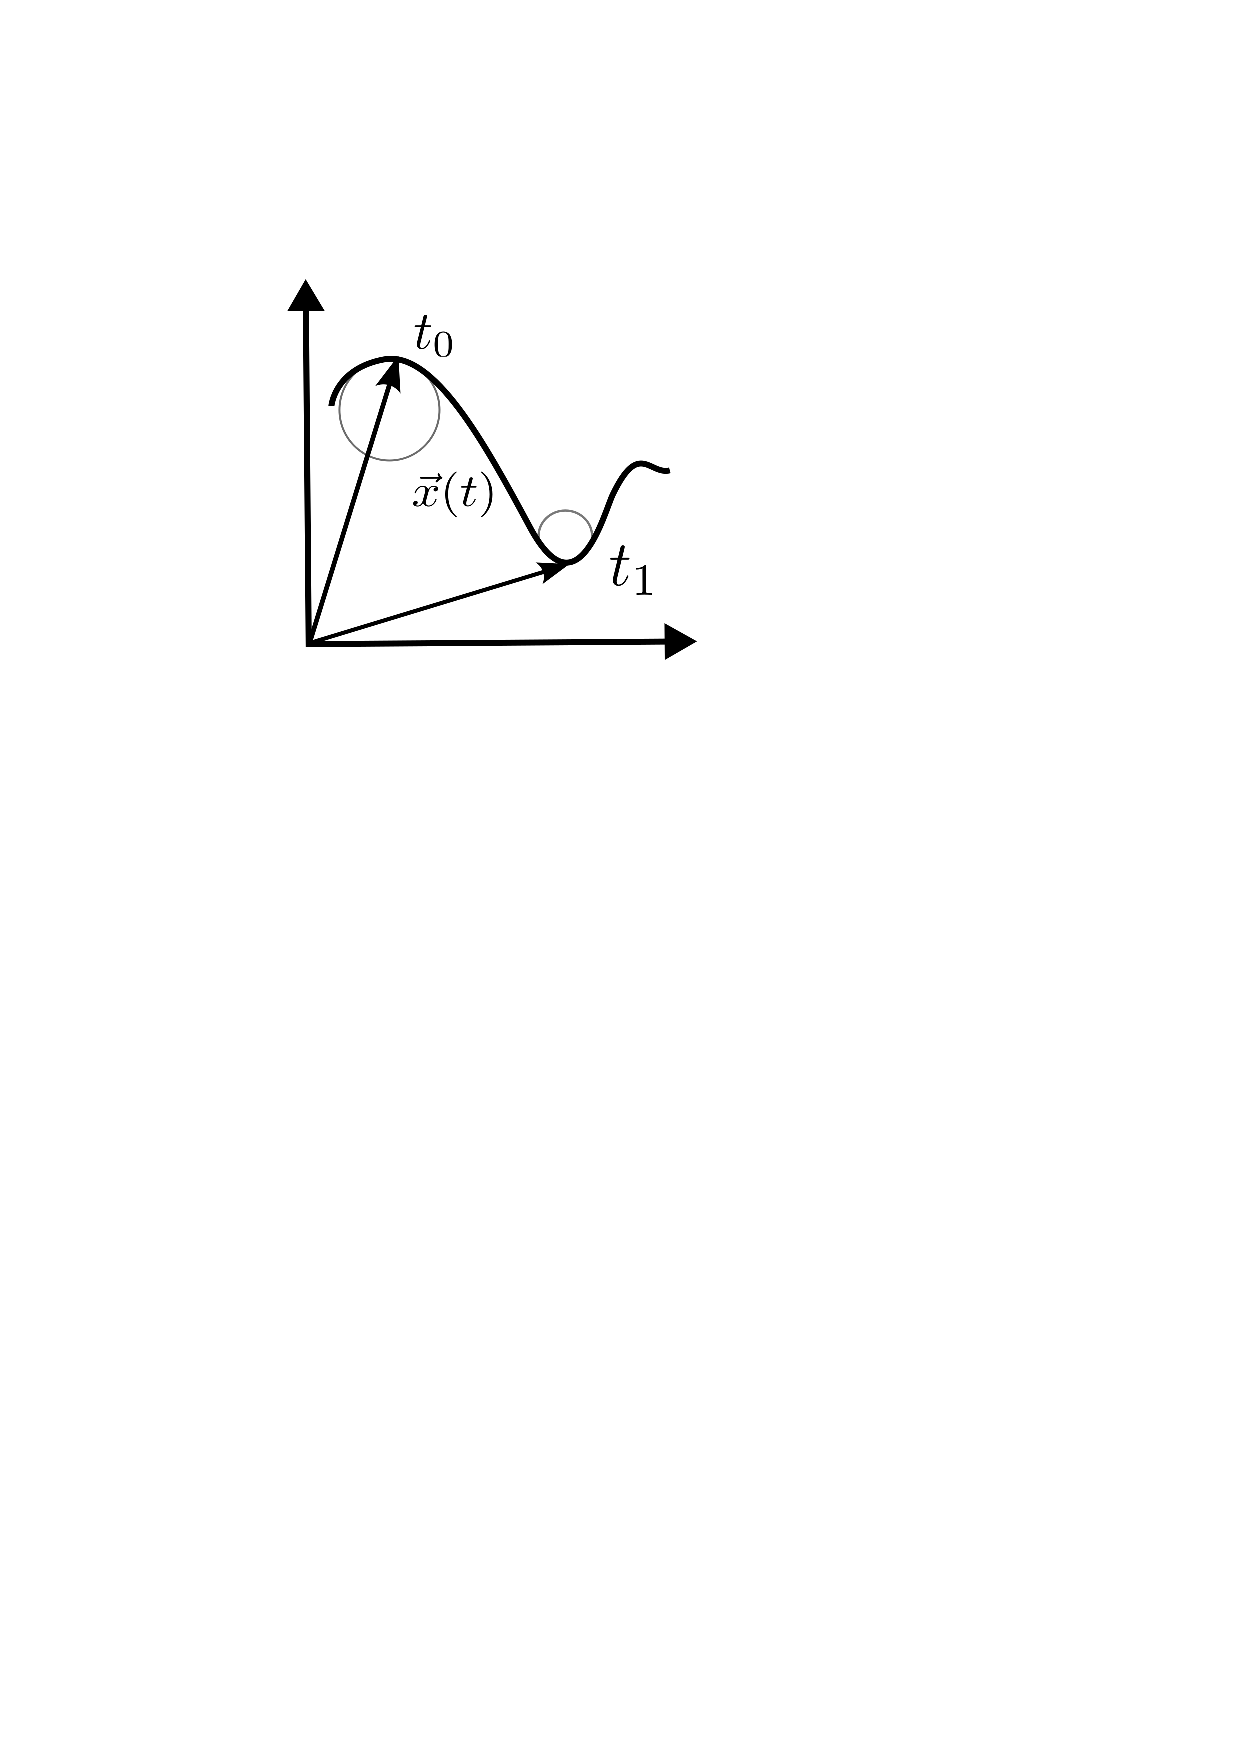
\includegraphics[scale=.4]{FOTOS/radio.png}
\end{wrapfigure}

Para el caso anterior de $x(t)=r\cos{t}, \  y(t)=r\sin{t}$; $\rho(t)=r\equiv$ constante. Geométricamente, $\rho(t)$ representa el \emph{radio instantáneo de una circunferencia} que aproxima \emph{cuadráticamente} la curva en un punto $t$.\\
\WFclear
\subsection{Sistema de Frenet en parametrización natural}

Dada nuestra curva $\mathbf{x}(S)=(x(S),y(S))$ en $\mathbb{R}^2$ en términos del parámetro privilegiado $S$, nuestro sistema de Frenet se construye de la siguiente forma:
\begin{equation*}
\begin{split}
    \left \{ \begin{array}{ccc}
      \mathbf{e_1}   &=&\dot{\mathbf{x}}(S)=(\dot{x}(S),\dot{y}(S))  \\
      \mathbf{e_2}   &=&(-\dot{y}(S),\dot{x}(S)) 
    \end{array} \right . \implies K(S)=\dot{\mathbf{e_1}}(S)\cdot \mathbf{e_2}(S)&=-\ddot{x}(S)\dot{y}(S)+\ddot{y}(S)\dot{x}(S)\\
                                                                     K(t)&=\dot{x}(S)\ddot{y}(S)-\ddot{x}(S)\dot{y}(S)
\end{split}
\end{equation*}
(Resulta más sencillo calcular la curvatura en parametrización natural).
\subsection{Interpretación geométrica de la curvatura en $\mathbb{R}^2$}
Sea $\mathbf{x}:I\subseteq\mathbb{R}\longrightarrow \mathbb{R}^2$ de clase $C^r\ , \ r\ge 2$, escrita en términos del parámetro natural.\\

\begin{wrapfigure}{l}{0.4\textwidth}  
    \centering
    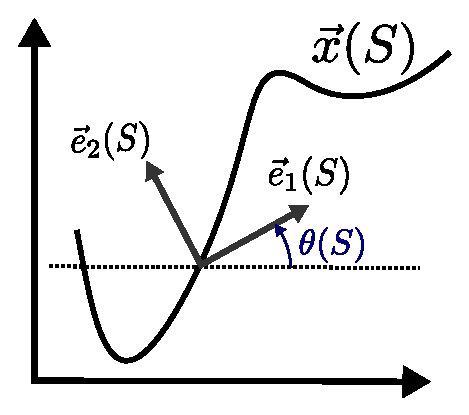
\includegraphics[scale=.8]{FOTOS/interpretacion.eps}
\end{wrapfigure}

$\theta (S)$ es el ángulo que forma el primer vector del sistema de Frenet, que coincide con $\dot{\mathbf{x}}(S)$, con el eje horizontal. Recordamos que estas derivadas en términos de $S$ cumplen que $||\dot{\mathbf{x}}(S)||=1$, por lo que 
$$
\dot{x}(S)^2+\dot{y}(S)^2=1
$$

Además, si descomponemos este vector velocidad en términos de sus proyecciones horizontales y verticales, obtenemos que
$$
\left \{ 
\begin{array}{ccc}
     \dot{x}(S)&=&\cos{\theta(S)}  \\
     \dot{y}(S)&=&\sin{\theta(S)} 
\end{array}
\right .
$$

Por lo que la curvatura $K(S)$ queda escrita como:
\begin{flalign*}
    K(S)&=\dot{x}\ddot{y}-\ddot{x}\dot{y}&&\\
        &=\cos{\theta(S)}\cdot \cos{\theta(S)}\cdot \dot{\theta}(S)+\sin{\theta(S)}\cdot \dot{\theta}(S)\cdot \sin{\theta(S)}=\dot{\theta}(\cos^2\theta + \sin^2\theta)&&\\
        &\implies \boxed{K(S)=\dot{\theta}(S)}
\end{flalign*}

La curvatura representa la variación del ángulo $\theta$ en términos de la longitud de arco.
\subsection{Reconstrucción de una curva a partir de su curvatura}
Supongamos que conocemos la curvatura $K(S)$ de una curva, donde $S$ es el parámetro natural. Recordemos que $K(S)=\dot{\theta}(S)$, con $\dot{x}=\cos{\theta}$, $\dot{y}=\sin{\theta}$. Entonces,
$$
\theta(S)=\int K(S) \odif{S} + \theta_0 \qquad \text{\parbox{10.5cm}{con una constante de integración asociada a la libertad de rotación.}}
$$
y
$$
\begin{array}{ccc}
     x(S)&=&\int \cos{\theta(S)} \odif{S} + x_0 \\
     y(S)&=&\int \sin{\theta(S)} \odif{S} + y_0
\end{array} \qquad \text{\parbox{9cm}{con $x_0,y_0$ constantes de integración asociadas a la libertad de traslación.}}
$$
\begin{mybox}
    \underline{Ejemplo I:} $K(S)=1/(1+S^2)$. Hallar la curva paramétrica.
    $$
    \theta(S)=\int K(S)\odif{S} = \int \frac{\odif{S}}{1+S^2}=\arctan{S}+\cancelto{0}{\theta_0}
    $$

    \begin{enumerate}
        \item[$\rightarrow$] $x(S)$:
        $$
        x(S)=\int \cos{\theta(S)}\odif{S}=\int \cos[\arctan S]\odif{S}
        $$ 

        Por trigonometría: $\tan{\alpha}=\sin{\alpha}/\cos{\alpha}=\sqrt{1-\cos^2\alpha}/\cos\alpha$, por lo que $\cos \alpha=\sqrt{1/(1+\tan^2 \alpha)}$
        $$
        x(S)=\int \cos[\arctan S]\odif{S}=\int \sqrt{\frac{1}{1+s^2}}\odif{S}=\sinh^{-1}(S)+\cancelto{0}{x_0}
        $$

        \item[$\rightarrow$] $y(S)$:
        \begin{flalign*}  
            y(S)&=\int \sin{\theta(S)}\odif{S}&&\\
                &=\int \sin{\arctan \theta}\odif{S}=\int \frac{S\odif{S}}{\sqrt{1+S^2}}=\sqrt{1+S^2}+\cancelto{0}{y_0}
        \end{flalign*}
    \end{enumerate}
    
    Finalmente:
    $$
    \left \{ 
    \begin{array}{ccc}
         x(S)&=&\sinh^{-1}(S)  \\
         y(S)&=&\sqrt{1+S^2} 
    \end{array}
    \right . 
    $$
     \begin{wrapfigure}{r}{0.25\textwidth} 
        \centering
        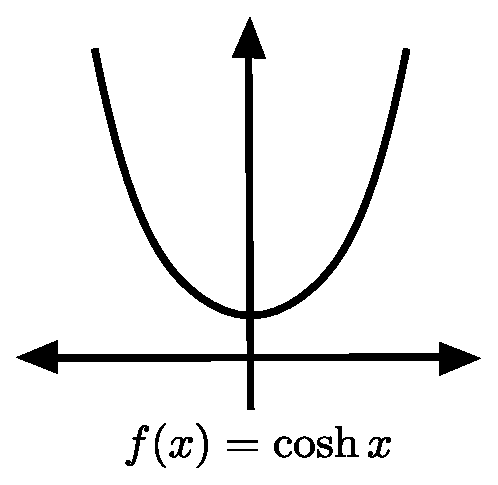
\includegraphics[scale=.45]{FOTOS/catenaria.eps}
    \end{wrapfigure}
    $$
    \mathbf{x}(S)=\left (\sinh^{-1}(S),\sqrt{1+S^2} \right )
    $$
   
    Representar esta curva mediante este parámetro es complicado, por lo que en este caso es útil utilizar una reparametrización.
    $$
    t=\sinh^{-1}(S)\implies \sinh{t}=S \ , \ \sqrt{1+S^2}=\cosh{t}
    $$
    
\end{mybox}

\section{Fórmulas de Frenet}
 Ya hemos tratado el problema del sistema de Frenet en dos dimensiones e introducido el concepto de curvatura a través de la parametrización natural. En el caso de $\mathbb{R}^3$, nuestro parámetro $S\in I$ define la curva como 
 $$
 S\longmapsto \mathbf{x}(S)=(x(S),y(S),x(S))
 $$
 y nuestro sistema de Frenet toma una forma sencilla, porque $||\dot{\mathbf{x}}(S)||=1$.
 $$
 \left \{
 \begin{array}{ccc}
      \mathbf{e_1}(S)&=&\dot{\mathbf{x}}(S)  \\
      \mathbf{e_2}(S)&=&\ddot{\mathbf{x}}(S)/||\ddot{\mathbf{x}}(S)||\\
      \mathbf{e_3}(S)&=&\mathbf{e_1}(S)\wedge \mathbf{e_2}(S)=\frac{\dot{\mathbf{x}}(S)\wedge \ddot{\mathbf{x}}(S)}{||\ddot{\mathbf{x}}(S)||}
 \end{array}
 \right .
 $$

 La notación clásica para el \emph{triedro de Frenet} es:
 \begin{center}
\begin{tabular}{cccc}
     $\mathbf{t}(S)=\mathbf{e_1}$ &:& Vector& \emph{tangente unitario}.\\
     $\mathbf{p}(S)=\mathbf{e_2}$ &:& Vector& \emph{normal principal}.\\
     $\mathbf{b}(S)=\mathbf{e_3}$ &:& Vector& \emph{binormal}.\\
\end{tabular}
\end{center}


\begin{wrapfigure}{l}{0.35\textwidth}
    \centering
    \includegraphics[scale=.4]{FOTOS/frenet_3d.png}
\end{wrapfigure}

Se puede ver de forma muy sencilla que, para $\mathbf{x}\in \mathbb{R}^3$ y un cierto $S$ fijo, $\mathbf{x}(S),\mathbf{t}(S),\mathbf{p}(S),\mathbf{b}(S)$ quedan totalmente fijados. Entonces, para ese punto de coordenadas $\mathbf{z}(S)=(x(S),y(S),z(S))$, los vectores del triedro de Frenet forman tres planos, llamados \emph{normal, rectificante }y \emph{osculador}, que quedan determinados respectivamente por:
$$
\begin{array}{c}
     (\mathbf{z}-\mathbf{x}(S))\cdot \mathbf{t}=0  \\
     (\mathbf{z}-\mathbf{x}(S))\cdot \mathbf{p}=0  \\
     (\mathbf{z}-\mathbf{x}(S))\cdot \mathbf{b}=0
\end{array}
$$
\begin{wrapfigure}{r}{0.3\textwidth}
    \centering
    \includegraphics[scale=.4]{FOTOS/planos_triedro.png}
\end{wrapfigure}
En el caso de una curva en $\mathbb{R}^3$, recordamos que tenemos dos curvaturas:
$$
\begin{array}{ccccc}
    K_1(S)&\equiv& \underbrace{K(S)}_{(>0)}  & :&\text{\underline{curvatura}}\\\\
    K_2(S)&\equiv &\tau(S)   &:& \text{\underline{torsión}}
\end{array}
$$

$$
\left ( \begin{array}{c}
     \dot{\mathbf{t}}(S)  \\
     \dot{\mathbf{p}}(S)  \\
     \dot{\mathbf{b}}(S)
\end{array} \right )=\left ( \begin{array}{ccc}
     0&K(S) &0 \\
     -K(S)&0 &\tau (S) \\
     0&-\tau (S) &0
\end{array} \right ) \left ( \begin{array}{c}
     \mathbf{t}(S)  \\
     \mathbf{p}(S)  \\
     \mathbf{b}(S)
\end{array} \right )
$$

La forma explícita de la curvatura y la torsión es:
\begin{enumerate}
    \item[(i)] $K(S)=K_1(S)=$
    $\dot{\mathbf{e}}_1(S)\cdot \mathbf{e}_2(S)=(\ddot{\mathbf{x}}(S)\cdot \ddot{\mathbf{x}}(S))/||\ddot{\mathbf{x}}(S)||=||\ddot{\mathbf{x}}(S)||>0$.
    $$
    \boxed{K(S)=||\ddot{\mathbf{x}}(S)||}
    $$ 

    \item[(ii)] $\tau(S)=K(S)=\dot{\mathbf{e}}_2(S)\cdot \mathbf{e}_3(S)$

    \begin{gather*}
        \mathbf{e_2}=\frac{\ddot{\mathbf{x}}}{||\ddot{\mathbf{x}}||}\implies \dot{\mathbf{e}}_2=\dddot{\mathbf{x}}(S)\cdot \frac{1}{||\ddot{\mathbf{x}}(S)||}+\ddot{\mathbf{x}}(S)\cdot \dv{}{S}\left ( \frac{1}{||\ddot{\mathbf{x}}||} \right ) \\
        \text{pero } \ddot{\mathbf{x}}(S)=\mathbf{e}_2\cdot ||\ddot{\mathbf{x}}(S)||
    \end{gather*}
    es decir, el término de la derivada del módulo no contribuye, quedando únicamente la tercera derivada.
    $$
    \tau(S)=\dot{\mathbf{e}}_2\cdot \mathbf{e}_3=\dot{\mathbf{e}}_2\cdot (\mathbf{e}_1 \wedge \mathbf{e}_2)=\frac{\dddot{\mathbf{x}}(S)}{||\ddot{\mathbf{x}}(S)||}\cdot (\mathbf{e}_1 \wedge \mathbf{e}_2)
    $$
    $$
    \boxed{\tau(S)=\frac{\det{\dot{\mathbf{x}},\ddot{\mathbf{x}},\dddot{\mathbf{x}}}}{||\ddot{\mathbf{x}}||^2}}
    $$
    luego tenemos que $||\ddot{\mathbf{x}}||\neq 0$
\end{enumerate}

Se define el \emph{vector de curvatura} como:
$$
\boxed{\mathbf{K}(S)=K(S)\cdot \mathbf{p}(S)} \ ,
$$
el \emph{centro de curvatura} (para cada punto de la curva) como:
$$
\boxed{\mathbf{x}_{cc}(S)=\mathbf{x}(S)+\frac{1}{K(S)}\mathbf{p}(S)}
$$
y el \emph{radio de curvatura} como:
$$
\boxed{\rho(S)=\frac{1}{K(S)}}
$$

Hasta este punto, todo este desarrollo se aplica para la parametrización natural, especialmente simple por la condición de $||\dot{\mathbf{x}}(S)||=1$. En casos de la parametrización \emph{arbitraria}, se arrastran términos de $||\dot{\mathbf{x}}(S)||=1$ debido a su no unitariedad.\\

En este caso, el triedro de Frenet es:
\begin{gather*}
    \mathbf{e}_1(t)=\frac{\mathbf{x'}(t)}{||\mathbf{x'}(t)||}\equiv \mathbf{t}(t)\\
    \mathbf{e}_3(t)=\frac{\mathbf{x'}(t)\wedge \mathbf{x''}(t)}{||\mathbf{x'}(t)\wedge \mathbf{x''}(t)||}\equiv \mathbf{b}(t)\\
    \mathbf{e}_2(t)=\mathbf{e}_3\wedge \mathbf{e}_1=\mathbf{b}(t)\wedge \mathbf{t}(t)\equiv \mathbf{p}(t)
\end{gather*}

Para calcular la curvatura y la torsión, recordamos que:
\begin{align*}
    K(S)=||\ddot{\mathbf{x}}(S)||&:&\text{\parbox{7cm}{Como se trata de un cambio de variable: $\dv*{}{S}=1/||\mathbf{x'}||\dv*{}{t}$}}
\end{align*}
\begin{enumerate}
    \item[$\xlongrightarrow{1}$]$\dot{\mathbf{x}}(S)=\dv{\mathbf{x}}{S}=\frac{1}{||\mathbf{x'}||}\dv{\mathbf{x}}{t}=\frac{\mathbf{x'}}{||\mathbf{x'}||}$ 

    \item[$\xlongrightarrow{2}$]$\ddot{\mathbf{x}}(S)=\dv{\dot{\mathbf{x}}}{S}=\frac{1}{||\mathbf{x'}||} \left ( \dv{}{t}\left ( \frac{\mathbf{x'}}{||\mathbf{x'}||} \right ) \right )=\frac{\mathbf{x''}}{||\mathbf{x'}||^2}+\mathbf{x'}\cdot \frac{1}{||\mathbf{x'}||} \dv{}{t}\left ( \frac{1}{||\mathbf{x'}||} \right )$
\end{enumerate}

Utilizando los cálculos anteriores,
$$
K(t)=\frac{||\mathbf{x'}(t)\wedge \mathbf{x''}(t)||}{||\mathbf{x'}(t)||^3} \qquad , \qquad \tau(t)=\frac{\det{\dot{\mathbf{x}},\ddot{\mathbf{x}},\dddot{\mathbf{x}}}}{||\mathbf{x'}(t)\wedge \mathbf{x''}(t)||^2}
$$

\subsection{Curvas planas en $\mathbb{R}^3$}
Una curva plana es aquella que está \emph{contenida en un plano} de $\mathbb{R}^3$. Eso significa que uno de los vectores del triedro de Frenet no se está moviendo, en este caso $\mathbf{b}(S)$; es decir, es \emph{constante}.

El trabajar con una curva plana hace que se cumpla que $(\mathbf{x}(S)-\mathbf{x}(0))\cdot \mathbf{n}=0$, donde $\mathbf{n}$ es un vector normal al plano que contiene la curva. Si derivamos esta expresión, obtenemos $\dot{\mathbf{x}}\cdot \mathbf{n}=0$, y $\ddot{\mathbf{x}}\cdot \mathbf{n}=0$, de donde podemos deducir que $\ddot{\mathbf{x}}\sim \mathbf{b} \implies \mathbf{m} \parallel \mathbf{b}(S)$. En consecuencia, $\mathbf{b}\equiv $ const., con $||\mathbf{b}(S)||=1$. \\

Por lo tanto, una curva (en $\mathbb{R}^3$) con curvatura distinta de 0 es plana si y solo si $\tau(S)$ es nula ($\dot{\mathbf{b}}(S)=-\tau(S)\mathbf{p}(S)\equiv 0 \iff \tau(S)=0$).
\begin{mybox}
    \begin{center}
    \fbox{\textbf{Condiciones equivalentes}} \\
    \vspace{0.3cm}
    Una curva es \textbf{plana} si y solo si:
    \begin{gather*}
        \mathbf{b}(S)\equiv \text{constante}
        \iff 
        (\mathbf{x}(S)-\mathbf{x}(0))\cdot \mathbf{n}=0
       \iff 
        \tau(S)=0
    \end{gather*}
    \end{center}
\end{mybox}

\begin{center}
    \includegraphics[scale=.65]{FOTOS/curva_plana.png}
\end{center}



\chapter{FIREBALL}
\section{Introducción al código FIREBALL}
Consiste en un procedimiento basado en el formalismo de electrones fuertemente ligados (\emph{tight-binding}) y de dinámica molecular, parametrizada con datos \emph{ab-initio}. Se procede a realizar un cálculo de DFT usando orbitales atómicos (LCAO) modificados para cortarlos a un determinado valor de la distancia al núcleo, a partir del cual la f.d.o se hace nula. \\

% \coffeestainD{0.5}{0.85}{-25}{5cm}{1.3cm} 

Por otro lado, se usa la aproximación de McWeeda para modelizar la energía de correlación y canje.
\section{Cálculos con FIREBALL: resultados}
\subsection{Grafeno 1x1: energías frente parámetro de red}
\begin{figure}[!h]
    \centering
    \includegraphics[scale=.8]{FIGURAS/En_param_graf1x1.png}
    \caption{$E$ (eV) frente a $a$ (\AA)}
    \label{fig:enter-label}
\end{figure}



El parámetro de red $a$ que tiene asociada la energía más pequeña es $a = 1.43 $ \AA, con $E_{TOT} = -307.207591$ eV.
\subsection{Densidad de estados frente a energía}
\begin{figure}[!h]
    \centering
    \includegraphics[scale=.6]{FIGURAS/Densidad_1.png}
    \caption{DOS frente a $E$ (eV)}
    \label{fig:enter-label}
\end{figure}
\begin{figure}[!h]
    \centering
    \includegraphics[scale=.6]{FIGURAS/Densidad_2.png}
    \caption{DOS frente a $E$ (eV)}
    \label{fig:enter-label2}
\end{figure}
\begin{figure}[!t]
    \centering
    \includegraphics[scale=.6]{FIGURAS/Densidad_total.png}
    \caption{DOS frente a $E$ (eV)}
    \label{fig:enter-label3}
\end{figure}
\clearpage 
\section{Grafeno 18x8. Estiramiento, energía y fuerzas}

% \begin{figure}[!h]
%     \centering
%     \includegraphics[scale = .9]{FIGURAS/E_desp_graf_18x8.png}
%     \label{fig:graf_18x8}
% \end{figure}

\begin{figure}[!h]
    \centering
    \includegraphics[scale = .9]{FIGURAS/E_F_desp_graf_18x8.png}
    \label{fig:18x8_e_ef}
\end{figure}

Rehacer las figuras

\begin{itemize}
    \item El grafeno se rompe por uno de los extremos. Es más estable romper por los extremos.
    \item Al realizar un estiramiento progresivo de la red, observamos que la configuración de mínima energía es muy distinta a la obtenida al estirar rígidamente por los extremos. 
\end{itemize}

\section{Grafeno 18x8 vacante y divacante}

\begin{itemize}
    \item Al haber una vacante, es más estable que el grafeno se rompa por el defecto antes que por la región en la que estiramos. 
    \item Ocurre lo mismo con la divacante. 
    \item En ambos casos, la configuración de mínima energía hace que los átomos de la región de ruptura salgan del plano del grafeno. 
\end{itemize}


\section{Conlusiones}

\begin{itemize}
    \item Importa el tipo de defecto que introducimos.
    \item Importa la manera en la que estiramos. 
\end{itemize}

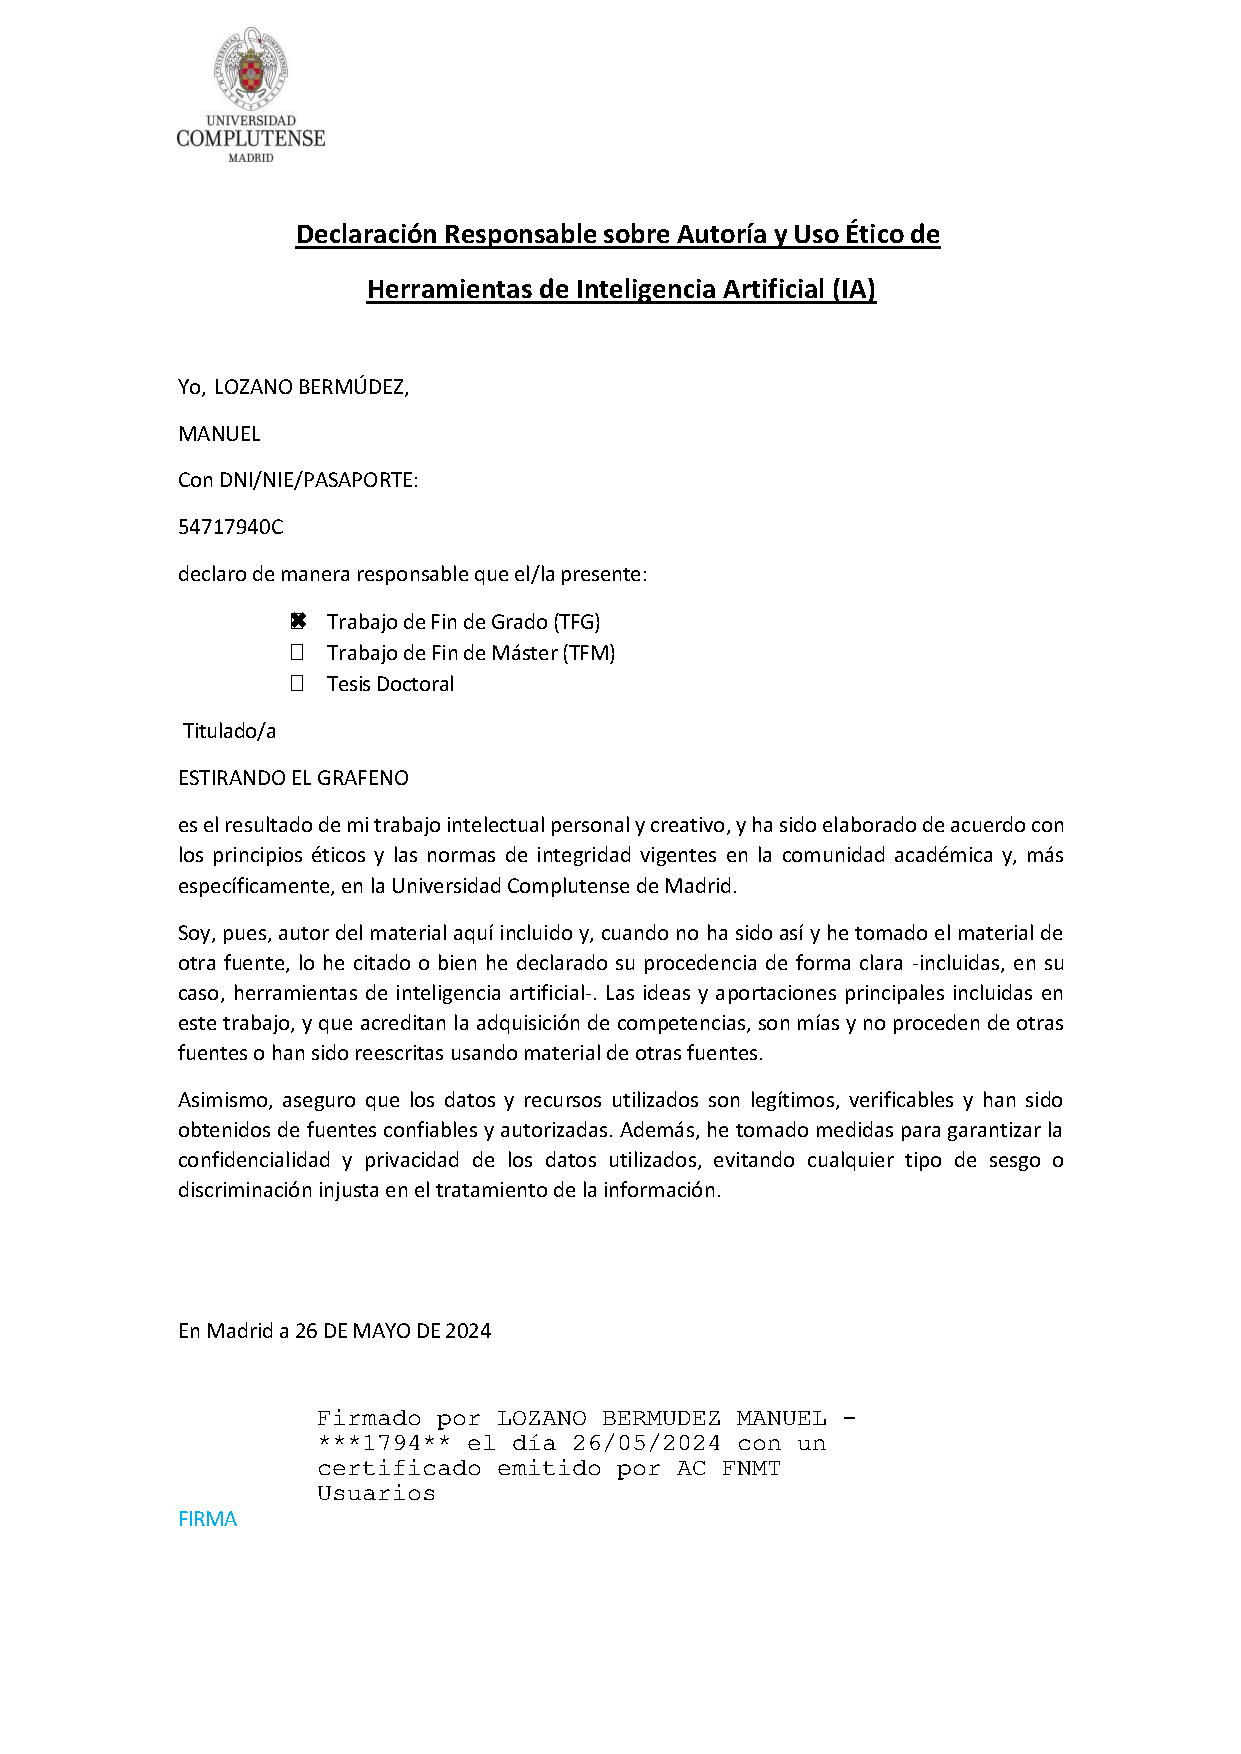
\includepdf{declaracion-responsable-sobre-autoria-y-uso-etico-de-ia_signed.pdf}

% \coffeestainA{0.9}{0.85}{-25}{5cm}{1.3cm}

\chapter{Segunda forma fundamental, curvatura media y gaussiana}

\section{Segunda forma fundamental}
\large 

Sea una superficie parametrizada $S$,
\begin{align*}
    \mathbf{x}:U\subseteq \mathbb{R}^2&\longrightarrow V\cap S\\
    (u^1,u^2)&\longmapsto \mathbf{x}(u^1,u^2) \ ,
\end{align*}
y un punto genérico de la superficie $S$, $P$. Además, sea $T_p(S)$ el espacio o plano tangente a $S$ en el punto $P$. En este punto $P$, el conjunto de vectores $\left \{ \mathbf{x}_1=\pdv{\mathbf{x}}{u^1},\mathbf{x}_2=\pdv{\mathbf{x}}{u^2} ,\mathbf{n}=\frac{\mathbf{x}_1\wedge \mathbf{x}_2}{||\mathbf{x}_1\wedge \mathbf{x}_2||}\right \}$ es una base de $\mathbb{R}^3$.\\

\begin{wrapfigure}{l}{0.3\textwidth}
    \centering
    \includegraphics[scale=.5]{FOTOS/curvatura_dist.png}
\end{wrapfigure}

Consideramos un punto $P^*\in S$ infinitesimalmente próximo al punto $P$, de tal modo que las coordenadas de $P$ y $P^*$ son, respectivamente, $(u^1,u^2),(u^1+h^1,u^+h^2)$. Para medir la curvatura, estudiaremos cuánto se separa la superficie $S$ de $T_p(S)$.
$$
d(P^*,T_p(S))=(\mathbf{x}(u^p+h^p)-\mathbf{x}(u^p))\cdot \mathbf{n}
$$

Como $P$ y $P^*$ están infinitamente cerca, podemos expandir en serie de Taylor:
$$
\mathbf{x}(u^p+h^p)=\mathbf{x}(u^p)+\mathbf{x}_\alpha \cdot h^\alpha +\frac{1}{2}\mathbf{x}_{\alpha \beta }(u^p)\cdot h^\alpha h^\beta +\mathbf{R}_2
$$
Por lo que la distancia queda como:
\begin{equation*}
    \begin{split}
        d(P^*,T_p(S))&=\left ( \mathbf{x}_\alpha(u^p)\cdot h^\alpha +\frac{1}{2}\mathbf{x}_{\alpha \beta }(u^p)\cdot h^\alpha h^\beta +\ldots   \right )\cdot \mathbf{n}\\
        &=\frac{1}{2}\mathbf{x}_{\alpha \beta }\cdot \mathbf{n}h^\alpha h^\beta \qquad \text{porque }\mathbf{x}_\alpha \cdot \mathbf{n}=0
    \end{split}
\end{equation*}
Al producto escalar de la segunda derivada con el vector perpendicular a $T_p(S)$ lo llamaremos \emph{segunda forma fundamental}.
$$\boxed{b_{\alpha \beta }=\mathbf{x}_{\alpha \beta }\cdot \mathbf{n}}$$

Otra manera alternativa de expresar la segunda forma fundamental se obtiene derivando la expresión $\mathbf{x}_\alpha \cdot \mathbf{n}=0$:
$$
\mathbf{x}_{\alpha \beta }\cdot \mathbf{n}+\mathbf{x}_\alpha \mathbf{n}_\beta =0 \implies \boxed{b_{\alpha \beta }=-\mathbf{x}_\alpha \cdot \mathbf{n}_\beta }
$$

Para el determinante de esta matriz, utilizaremos la notación $b=\det{b_{\alpha \beta }}$. El nombre de segunda forma fundamental proviene de que la distancia $d(P^*,T_p(S))=1/2b_{\alpha \beta }h^\alpha h^\beta +\ldots $ es, a orden dominante, una forma cuadrática:
$$
Q(h^\alpha )=\frac{1}{2}b_{\alpha \beta }h^\alpha h^\beta 
$$

No obstante, al contrario que de la primera forma fundamental, esta \emph{no} tiene porqué ser definida positiva. 
\begin{mybox}
    \begin{center}
        \textbf{SEGUNDA FORMA FUNDAMENTAL}
    \end{center}
    $$
    b_{\alpha \beta }=\mathbf{x}_{\alpha \beta }\cdot \mathbf{n}=-\mathbf{x}_\alpha \cdot \mathbf{n}_\beta 
    $$
    \textbf{Propiedades:}
    \begin{enumerate}
        \item Si $b_{\alpha \beta }=0$ sobre una cierta carta local, la superficie en esa carta es un \textbf{plano}, y viceversa.
        \item $b_{\alpha \beta} $ son las componentes covariantes de un (pseudo-)tensor de segundo orden.
        \item La ley de transformación de $b$ es $\Bar{b}=D^2b$.
    \end{enumerate}
\end{mybox}
\begin{enumerate}
    \item[\fbox{1}] 
    \begin{proof}
            Suponemos que $b_{\alpha \beta }=0$, y sabemos que $||\mathbf{n}||=1 \leftrightarrow \mathbf{n}\cdot \mathbf{n}=1$. Derivando: $\mathbf{n}_\alpha \cdot \mathbf{n}+\mathbf{n} \cdot \mathbf{n}_\alpha\implies \mathbf{n}\cdot \mathbf{n}_\alpha =0 \iff \mathbf{n}_\alpha \in T_p(S)$. Esto significa que $\mathbf{n}_\alpha $ puede expresarse como combinación lineal de la base $\{ \mathbf{x}_1,\mathbf{x}_2 \} $. Por tanto:
            $$
            \left \{ \begin{array}{c}
                 b_{\alpha \beta }=0  \\
                 \mathbf{n}_\alpha \in T_p(S) 
            \end{array} \right . \implies \mathbf{x}_\alpha \cdot \mathbf{n}_\beta =0\iff \mathbf{n}\equiv \text{const.} 
            $$
            Entonces:
            $$
            (\mathbf{x}\cdot \mathbf{n})_\alpha =\cancelto{0}{\mathbf{n}\cdot \mathbf{x}_\alpha }+\cancelto{0}{\mathbf{n}_\alpha \cdot \mathbf{x}}
            $$
            Luego:
            $$
            \mathbf{x}\cdot \mathbf{n}\equiv \text{const.}\qquad \text{Ecuación de un plano.} 
            $$
    \end{proof}
    \item[\fbox{2}]
    \begin{proof}
        Si cambiamos de coordenadas $u^\alpha $ a $\Bar{u}^\beta $:
        \begin{equation*}
        \begin{split}
            \Bar{\mathbf{n}}=\frac{\Bar{\mathbf{x}}_1\wedge \Bar{\mathbf{x}}_2}{||\Bar{\mathbf{x}}_1\wedge \Bar{\mathbf{x}}_2||}\longrightarrow \Bar{b}_{\alpha \beta }=-\Bar{\mathbf{x}}_\alpha \cdot \Bar{\mathbf{n}}_\beta &=-\left ( \pdv{u^\mu }{\Bar{u}^\alpha } \mathbf{x}_\mu \right ) \cdot \left ( \pdv{u^\nu }{\Bar{u}^\beta } \mathbf{n}_\nu \right )\\
            &=- \pdv{u^\mu }{\Bar{u}^\alpha }\pdv{u^\nu }{\Bar{u}^\beta }\underbrace{\mathbf{x}_\mu\cdot \mathbf{n}_\nu}_{-b_{\mu \nu }}\\
            &=\pdv{u^\mu }{\Bar{u}^\alpha }\pdv{u^\nu }{\Bar{u}^\beta }b_{\mu \nu }
        \end{split}
        \end{equation*}
    \end{proof}
\end{enumerate}
\subsection{Clasificación de los puntos de una superficie}
Dada la superficie $S$, el plano tangente $T_p(S)$ y el punto $P^*$ de la superficie infinitesimalmente cerca de $P$, podemos clasificar las superficies en función de las diferentes separaciones del plano tangente.
\begin{itemize}
    \item \underline{PUNTO ELÍPTICO}: Si $b>0$, la superficie se comporta localmente como un paraboloide de revolución (o elíptico).
    $$
    Q(h^\alpha )=\frac{1}{2}b_{\alpha \beta }h^\alpha h^\beta 
    $$
    Además, si $b_{11}>0$, la superficie está orientada en el sentido de $\mathbf{n}$ (como el paraboloide elíptico, por ejemplo).\\
    Por el contrario, si $b_{11}<0$, la superficie está orientada en el sentido contrario a $\mathbf{n}$.

    \item \underline{PUNTO HIPERBÓLICO}: Si $b<0$, la superficie se comporta localmente como un paraboloide hiperbólico (punto de silla).
    \item \underline{PUNTO PARABÓLICO}: Si $b=0$ pero $b_{\alpha \beta }\neq 0$, la superficie se comporta localmente como un cilindro parabólico.
\end{itemize}

    \begin{wrapfigure}{r}{.3\textwidth}
    \centering
        \includegraphics[scale=.3]{FOTOS/punto_parabolico.png}
        \caption*{Cilindro parabólico}
    \end{wrapfigure}
Si $b_{\alpha \beta}=0$ (es decir, la segunda forma fundamental se anula), entonces no podemos conocer la forma local de la superficie. En este caso, es necesario tomar el siguiente orden de aproximación en el desarrollo en serie de Taylor. A este tipo de puntos se les conoce como \underline{PUNTOS PLANARES}.\\

\WFclear
\begin{mybox}
\begin{wrapfigure}{r}{.36\textwidth}
        \centering
        \includegraphics[scale=.3]{FOTOS/ejemplo3_A.png}
        \caption*{Gráfica de $f(x,y)=x^2+y^3$}
    \end{wrapfigure}
 \underline{Ejemplo A:} $\mathbf{x}(u^1,u^2)=(u^1,u^2,(u^1)^2+(u^2)^3)$
    
    $$\mathbf{x}_1=(1,0,2u^1),\ \mathbf{x}_2=(0,1,3(u^2)^2)$$
    $$
    \mathbf{n}=\frac{\mathbf{x}_1\wedge \mathbf{x}_2}{||\mathbf{x}_1\wedge \mathbf{x}_2||}=\frac{(-2u^1,-3(u^2)^2,1)}{\sqrt{1+(u^1)^2+9(u^2)^4}}
    $$
    $$
    b_{\alpha \beta }=\mathbf{x}_{\alpha \beta }\cdot \mathbf{n}
    $$
    $\implies 
    \left \{ \begin{array}{ccccc}
         \mathbf{x}_{11}&=&(0,0,2)&&  \\
         \mathbf{x}_{12}&=&(0,0,0)&=&\mathbf{x}_{21}\\
         \mathbf{x}_{22}&=&(0,0,6u^2)&&
    \end{array} \right .
    $\\
    $
    \implies \left \{ \begin{array}{ccccc}
         b_{11}&=&\frac{2}{\sqrt{1+(u^1)^2+9(u^2)^4}}&&  \\
         b_{12}&=&0&=&b_{21}\\
         b_{22}&=&\frac{6u^2}{\sqrt{1+(u^1)^2+9(u^2)^4}}&&\\
    \end{array} \right .\\
    $\WFclear$  \text{Es decir: \quad \parbox{8cm}{$b>0$ si $u^2>0$: puntos elípticos\\
                                                                 $b<0$ si $u^2<0$: puntos hiperbólicos\\
                                                                 $b=0$ si $u^2=0$: puntos parabólicos}}$
\end{mybox}

\section{Curvaturas principales, media y gaussiana}
\begin{wrapfigure}{l}{.35\textwidth}
    \centering
    \includegraphics[scale=.26]{FOTOS/cpmg_1.png}
    \includegraphics[scale=.35]{FOTOS/cpmg_2.png}
\end{wrapfigure}
La curvatura de una curva contenida dentro de una superficie dependerá de la propia curva y de la curvatura de la superficie. Como ejemplo, podemos pensar en una circunferencia contenida en un plano, o la misma circunferencia entendida como el ecuador de una esfera. \\

La contribución a la curvatura de la curva que proviene de la superficie se debe a cómo varía el vector normal sobre la superficie y, en concreto, del ángulo que forman entre $\mathbf{n}$ y $\mathbf{k}$, con $\mathbf{k}=k\cdot \mathbf{p}$, donde $\mathbf{p}$ es el vector normal principal de la curva. Para ver esto, descompondremos $\mathbf{k}$, el vector de curvatura, en una componente \emph{normal} (o paralela a $\mathbf{n}$); y en otra no paralela.\\
$$
\mathbf{k}=\mathbf{k}_n+\mathbf{k}_g \qquad \qquad \mathbf{k}_n\cdot \mathbf{n}=0 \ (\mathbf{k}_n\parallel \mathbf{n})
$$
$\mathbf{k}_g$ será entonces el vector de curvatura \emph{geodésica} (debida al tipo de curva). \\

Sea $S$ una superficie parametrizada, y $C$ una determinada curva en $S$, parametrizada en términos de la longitud de arco ($||\dot{\mathbf{x}}(S)||=1)$.
$$
\mathbf{k}_n=k_n\cdot \mathbf{n} \qquad \text{y} \qquad k_n=\mathbf{k}\cdot \mathbf{n}
$$
Como $\mathbf{k}$, para una curva en parámetro natural, es $\mathbf{k}=\dot{\mathbf{t}}=\ddot{\mathbf{x}}$; al aplicar la regla de la cadena queda:
\begin{gather*}
    \ddot{\mathbf{x}}=\pdv{\mathbf{x}}{u^\alpha }\dot{u}^\alpha =\mathbf{x}_{\alpha \beta }\dot{u}^\alpha \dot{u}^\beta +\mathbf{x}_\alpha \ddot{u}^\alpha \\
    \implies k_n=\ddot{\mathbf{x}}\cdot \mathbf{n}=(\mathbf{x}_{\alpha \beta }\dot{u}^\alpha \dot{u}^\beta +\mathbf{x}_\alpha \ddot{u}^\alpha)\cdot \mathbf{n}=b_{\alpha \beta }\dot{u}^\alpha \dot{u}^\beta 
\end{gather*}
En el caso de encontrarnos en una parametrización arbitraria:
$$
\dot{u}^\alpha =\dv{u^\alpha }{S}=\dv{u^\alpha }{t}\cdot \dv{t}{S}=(u^\alpha )'\cdot \frac{1}{||\mathbf{x}'(t)||}
$$
De esta forma, 
$$
k_n=\frac{1}{||\mathbf{x}'(t)||^2}b_{\alpha \beta }(u^\alpha )'(u^\beta)'=\boxed{\frac{b_{\alpha \beta }(u^\alpha )'(u^\beta )'}{g_{\mu \nu }(u^\mu )'(u^\nu )'}=k_n}
$$

La \emph{curvatura normal} es el cociente entre la segunda y la primera forma fundamental, evaluadas sobre la curva (conocidas $u^\alpha =u^\alpha (t)$). La curvatura normal es, en realidad, el ángulo entre $\mathbf{n}$ y el vector de curvatura $\mathbf{k}$ (o $\mathbf{p}$). \\
\newpage
\begin{wrapfigure}{r}{.35\textwidth}
    \centering
    \includegraphics[scale=.37]{FOTOS/curva_normal.png}
\end{wrapfigure}
La curvatura de cada curva $C_i$ (las cuales pasan todas por el mismo punto), serán distintas, como aparece en la imagen. Para ello, definiremos las curvaturas normales principales de la superficie $S$ en el punto $P$.\\

\subsection{Curvaturas normales principales (de $S$ en $P$)}
Se definen como los valores mayor y menor de la curvatura normal para todas las curvas contenidas en esa superficie $S$ y que pasan por el punto $P$.\\

Por comodidad, introducimos la siguiente notación:
\paragraph{Notación:} $(u^\alpha )'=\dv{u^\alpha (t)}{t}=\ell ^\alpha \implies k_n=\frac{b_{\alpha \beta }\ell ^\alpha \ell ^\beta }{g_{\mu \nu }\ell ^\mu \ell ^\nu }=\frac{A}{B}$, con $A=b_{\alpha \beta }\ell ^\alpha \ell ^\beta $ y $B=g_{\mu \nu} \ell ^\mu \ell ^\nu $.\\

Para hallar los valores de $k_n$ máximos y mínimos, derivamos la curvatura normal e imponemos que sea nula.
$$
\pdv{k_n}{\ell ^\alpha }=0=\frac{B\pdv*{A}{\ell ^\alpha }-A\pdv*{B}{\ell ^\alpha }}{B^2}
$$
Si multiplicamos por $B$ y usamos que $k_n=A/B$, entonces la expresión anterior puede escribirse como:
$$
\pdv{A}{\ell^\alpha }-k_n\pdv{B}{\ell ^\alpha }=0
$$
y, junto con las expresiones explícitas de $A$ y $B$, llegamos a que:
$$
(b_{\alpha \beta }l^\beta +b_{\beta \alpha }\ell ^\beta )-k_n(g_{\alpha \beta }\ell ^\beta +g_{\beta \alpha }\ell ^\beta )=0
$$
Como $g_{\alpha \beta }$ y $b_{\alpha \beta}$ son simétricas en $\alpha $ y $\beta $, la expresión se simplifica:
\begin{gather*}
    (b_{\alpha \beta }-k_ng_{\alpha \beta})\ell ^\beta =0 \quad (\alpha ,\beta =1,2)\\
    \left .\begin{array}{cc}
         \alpha =1:&(b_{11}-k_ng_{11})\ell ^1+(b_{12}-k_ng_{12})\ell^2=0  \\
         \alpha =2:&(b_{21}-k_ng_{21})\ell ^1+(b_{22}-k_ng_{22})\ell^2=0
    \end{array} \right \} 
\end{gather*}
que es un sistema homogéneo con $(\ell^1,\ell^2)\neq (0,0)$. Por tanto, para las soluciones no triviales, el determinante de la matriz de coeficientes debe de ser nulo.
$$
\left | \begin{array}{cc}
     b_{11}-k_ng_{11}&b_{12}-k_ng_{12}  \\
     b_{21}-k_ng_{21}&b_{22}-k_ng_{22} 
\end{array} \right |=0
$$
Esta condición proporciona una ecuación con dos soluciones para $k_n$. Estas dos soluciones, que etiquetaremos $k_1$ y $k_2$ ($k_1\ge k_2$), se conocen como las \emph{curvaturas normales principales} de la superficie $S$ en el punto $P$.\\

Para calcular las curvaturas normales $k_1$ y $k_2$, introduciremos el \emph{operador de Weingarten}, que es la segunda forma fundamental con un índice covariante y otro contravariante.
$$
b^\mu {}_\nu \equiv \text{operador de Weingarten.}
$$
De la ecuación $(b_{\alpha \beta }-k_ng_{\alpha \beta})\ell ^\beta =0$, tenemos que 
\begin{gather*}
    g^{\alpha \mu}(b_{\alpha \beta }-k_ng_{\alpha \beta})\ell ^\beta =0\\
    \implies (b^\mu {}_\beta -k_n \delta ^\mu {}_\beta )\ell ^\beta =0\\
    \implies \left | \begin{array}{cc}
        b^1{}_1-k_n &b^1{}_2  \\
         b^2{}_1&b^2{}_2-k_n 
    \end{array} \right |=0
\end{gather*}
(que es una ecuación de autovalores para el operador de Weingarten). Desarrollando: 
$$
k_n^2-(b^1{}_1+b^2{}_2)k_n+(b^1{}_1b^2{}_2-b^2{}_1b^1{}_2)=0
$$
Si usamos que $b^1{}_1+b^2{}_2=b^\alpha {}_\alpha $ y que $\det(b^\mu {}_\nu )=\det(g^{\mu \alpha }b_{\alpha \nu})=\det(g^{\mu \nu })\det(b_{\alpha \nu})=b/g$, obtenemos la siguiente expresión:
$$
\boxed{k_n^2-b^\alpha {}_\alpha k_n+\frac{b}{g}=0}
$$

Las ecuaciones algebraicas de segundo grado pueden escribirse en términos de sus soluciones.
\begin{gather*}
    (k_n-k_1)(k_n-k_2)=0\\
    =k_n^2-(k_1+k_2)k_n+k_1k_2=0\\
    \implies k_1k_2=\frac{b}{g} \qquad k_1+k_2=b^\alpha {}_\alpha 
\end{gather*}

Y, finalmente, usando estas relaciones, podemos definir dos curvaturas para la superficie:
\begin{mybox}
    \begin{center}
        \textbf{CURVATURA MEDIA}
    \end{center}
    $$
    H\equiv \frac{1}{2}(k_1+k_2)=\frac{1}{2}b^\alpha {}_\alpha 
    $$
    Esta curvatura depende tanto de la primera forma fundamental como de la segunda forma fundamental.
    \begin{center}
        \textbf{CURVATURA GAUSSIANA}
    \end{center}
    $$
    K\equiv k_1\cdot k_2=\frac{b}{g}
    $$
    Al contrario de la curvatura media, esta curvatura \textbf{sólo depende de la primera forma fundamental}, al poder escribirse el determinante $b$ en términos de $g$.
\end{mybox}

A partir de esta definición, se dice que una superficie es \emph{minimal} si $H=0$ en todos sus puntos (el nombre se debe a que este tipo de superficies pueden probarse que tienen área mínima. Este es el caso del plano). Veamos cómo se transforman estas dos cantidades $H$ y $K$ bajo cambios de coordenadas. 

Como $b_{\alpha \beta }$ es un pseudo-tensor y $g_{\alpha \beta }$ es un tensor, $k_n$ sólo cambiará de signo si cambia el sentido de $\mathbf{n}$. Por tanto, el producto de $k_1k_2=K$ será \emph{invariante} bajo cambios de coordenadas. En consecuencia, la curvatura gaussiana $K$ es un \emph{escalar}. (también puede verse este hecho con las leyes de transformación tensoriales).
\section{Fórmulas de Weingarten y de Gauss. Símbolos de Christoffel}
Como hemos visto en el capítulo 1, el sistema de Frenet se adapta a la geometría de la curva que estudiamos (se desplaza con el parámetro $t$). La evolución de este sistema da lugar a la noción de curvaturas de una curva en $\mathbb{R}^n$. \\

En el caso de las superficies, escribiremos $\{ \mathbf{x}_{\alpha \beta },\mathbf{n}_\beta  \}$ en términos de $\{ \mathbf{x}_\alpha ,\mathbf{n} \}$, con $\alpha ,\beta =1,2$. Derivaremos los vectores $\{ \mathbf{x}_1,\mathbf{x}_2,\mathbf{n} \}$ con respecto a las coordenadas curvilíneas locales, 
$$
\mathbf{x}_{\alpha \beta }=\partial_\beta \mathbf{x}_\alpha =\Gamma_{\alpha \beta }{}^\gamma \mathbf{x}_\gamma +a_{\alpha \beta }\mathbf{n}
$$
$$
\mathbf{n}_\beta =\partial_\beta \mathbf{n}=c_\beta {}^\gamma \mathbf{x}_\gamma +d_\beta \mathbf{n}
$$
donde $\Gamma_{\alpha \beta}{}^\gamma ,a_{\alpha \beta} ,c_\beta ,d_\beta $ son los coeficientes. Analizamos primero la segunda ecuación: como $||\mathbf{n}||^2=\mathbf{n}\cdot \mathbf{n}=1,\ \mathbf{n}_\beta \cdot \mathbf{n}=0 \implies d_\beta =0$. 

Si usamos la base dual,
\begin{gather*}
    \mathbf{x}^\gamma \cdot \mathbf{n}_\beta =g^{\gamma \rho} \mathbf{x}_\rho \cdot \mathbf{n}_\beta=-g^{\gamma \rho} b_{\rho \beta }=-b^\gamma {}_\beta \\
    \implies \mathbf{x}^\gamma \cdot \mathbf{n}_\beta =c_\beta {}^\gamma =-b_\beta {}^\gamma 
\end{gather*}

De la primera ecuación, $\mathbf{n}\cdot \mathbf{x}_{\alpha \beta}=a_{\alpha \beta }$. Por definición, $b_{\alpha \beta }=\mathbf{n}\cdot \mathbf{x}_{\alpha \beta }$, de modo que $\mathbf{n}\cdot \mathbf{x}_{\alpha \beta }=a_{\alpha \beta }=b_{\alpha \beta }$. 

Si utilizamos la base dual, $\mathbf{x}^\gamma \cdot \mathbf{x}_{\alpha \beta }=\boxed{\Gamma _{\alpha \beta }{}^\gamma} $. Estas cantidades se conocen como los \emph{símbolos de Christoffel de segunda especie} (no son tensores). Los símbolos de Christoffel \emph{de primera especie} son:
$$
\Gamma _{\alpha \beta \gamma }=\mathbf{x}_\gamma \cdot \mathbf{x}_{\alpha \beta }=g_{\mu \gamma }\Gamma ^\mu{}_{\alpha \beta }
$$

La notación usada en la literatura matemática es $\Gamma _{\alpha \beta }{}^\gamma $. En física--y, en concreto, en Relatividad General-- usamos la notación $\Gamma ^\gamma {}_{\alpha \beta }$. \\

Con esta definición, las ecuaciones anteriores pueden escribirse como:
\begin{align}
    \mathbf{x}_{\alpha \beta }&=\Gamma _{\alpha \beta }{}^\gamma \mathbf{x}_\gamma +b_{\alpha \beta }\mathbf{n} &&\text{: Ecuación de Gauss} \tag*{[G]} \label{gauss}\\
    \mathbf{n}_\beta &=-b_\beta {}^\gamma \cdot \mathbf{x}_\gamma &&\text{: Ecuación de Weingarten} \tag*{[W]} \label{weingarten}
\end{align}
$$
b_{\alpha \beta }=\mathbf{n}\cdot \mathbf{x}_{\alpha \beta } \qquad \qquad \Gamma _{\alpha \beta }{}^\gamma =\mathbf{x}^\gamma \cdot \mathbf{x}_{\alpha \beta }
$$
\section{Propiedades de los símbolos de Christoffel}
\subsection{Simetrías}
Del \emph{teorema de Schwarz} \footnote{Básicamente, si $f(x,y)$ es continua en su dominio abierto $D$ y es de clase $C^2$, entonces $f_{xy}=f_{yx}$.}, $\mathbf{x}_{\alpha \beta }=\mathbf{x}_{\beta \alpha }$, con $\alpha ,\beta =1,2$, luego los símbolos de Christoffel, $\Gamma _{\alpha \beta }{}^\gamma =\mathbf{x}^\gamma \cdot \mathbf{x}_{\alpha \beta }$ son simétricos bajo el intercambio de $\alpha $ y $\beta $.
$$
\Gamma _{\alpha \beta }{}^\gamma =\Gamma _{\beta \alpha  }{}^\gamma 
$$
Esto significa que, de los $2\times 2\times 2=8$ símbolos posibles en un superficie, sólo 6 de ellos son independientes (en dimensión $n$, serían $n^2(n+1)/2$).\\

Gracias a esta simetría, es posible obtener los símbolos de Christoffel en términos de derivadas de la primera forma fundamental. Esta expresión será la definición más común para estos símbolos. \\

Habíamos definido la primera forma fundamental como:
$$
g_{\alpha \lambda }=\mathbf{x}_\alpha \cdot \mathbf{x}_\lambda ,\ \text{con }\alpha ,\lambda=1,2.
$$
Si derivamos con respecto a $u^\beta $:
\begin{equation} \label{[*]}\tag*{[*]}
    \begin{split}
        \pdv{g_{\alpha \lambda  }}{u^\beta }&=\mathbf{x}_{\alpha \beta }\cdot \mathbf{x}_\lambda +\mathbf{x}_\alpha \cdot \mathbf{x}_{\lambda \beta }\\
        &=\Gamma_{\alpha \beta \lambda }+\Gamma _{\lambda \beta \alpha }
    \end{split}
\end{equation}
Si ahora rotamos los índices cíclicamente: $\alpha \rightarrow \beta \rightarrow \lambda \rightarrow \alpha $
\begin{equation} \label{[**]}
    \pdv{g_{\beta \alpha }}{u^\lambda }=\Gamma _{\beta \lambda }+\Gamma _{\alpha \lambda \beta } \tag*{[**]}
\end{equation}
\begin{equation}\label{[***]}
    \pdv{g_{\lambda \beta }}{u^\alpha }=\Gamma _{\lambda \alpha \beta }+\Gamma _{\beta \alpha \lambda }\tag*{[***]}
\end{equation}
Si ahora calculamos \ref{[*]}+\ref{[***]}-\ref{[**]}:
$$
\pdv{g_{\alpha \lambda  }}{u^\beta }+\pdv{g_{\lambda \beta }}{u^\alpha }-\pdv{g_{\beta \alpha }}{u^\lambda }=2\Gamma _{\alpha \beta \lambda }
$$
Por lo que, finalmente, podemos escribir:
$$
\boxed{\Gamma _{\alpha \beta \lambda }=\frac{1}{2}\left ( \pdv{g_{\alpha \lambda  }}{u^\beta }+\pdv{g_{\lambda \beta }}{u^\alpha }-\pdv{g_{\beta \alpha }}{u^\lambda } \right )}
$$
que es la definición para los símbolos de Christoffel de primera especie. \\

Para los símbolos de Christoffel de segunda especie, usamos la primera forma fundamental en notación contravariante.
\begin{mybox}
    \begin{center}
        \textbf{DEFINICIÓN DE SÍMBOLOS DE CHRISTOFFEL}
    \end{center}
    De primera especie:
    $$
    \Gamma _{\alpha \beta \lambda }=\frac{1}{2}\left ( \pdv{g_{\alpha \lambda  }}{u^\beta }+\pdv{g_{\lambda \beta }}{u^\alpha }-\pdv{g_{\beta \alpha }}{u^\lambda } \right )
    $$
    De segunda especie:
    $$
    \Gamma _{\alpha \beta }{}^\mu =g^{\mu \lambda }\Gamma _{\alpha \beta \lambda }=\frac{1}{2}g^{\mu \lambda }\left ( \pdv{g_{\alpha \lambda  }}{u^\beta }+\pdv{g_{\lambda \beta }}{u^\alpha }-\pdv{g_{\beta \alpha }}{u^\lambda } \right )
    $$
    \noindent\rule{\textwidth}{0.5pt}
    \underline{Ejemplo B:}
    \begin{enumerate}
        \item[(i)] Símbolos de Christoffel para coordenadas ortogonales sobre una superficie $S$.
        $$
        g_{\alpha \beta }=g_{\alpha \beta }(u^1,u^2)=\left ( \begin{array}{cc}
             g_{11}&  \\
             & g_{22}
        \end{array} \right )\rightarrow g^{\alpha \beta }=\left ( \begin{array}{cc}
             1/g_{11}&  \\
             & 1/g_{22}
        \end{array} \right )
        $$
        Los símbolos de Christoffel son $\Gamma _{11}{}^1=g^{1\lambda }\Gamma _{11\lambda }$.
        \begin{equation*}
            \begin{split}
                \Gamma _{11}{}^1&=g^{11}\Gamma_{111}+\cancel{g^{12}\Gamma _{112}}=\frac{1}{2g_{11}}\left ( \pdv{g_{11}}{u^1}+\cancel{\pdv{g_{11}}{u^1}}-\cancel{\pdv{g_{11}}{u^1}} \right )\\
                &=\frac{1}{2g_{11}}\pdv{g_{11}}{u^1}(u^1,u^2)
            \end{split}
        \end{equation*}
        \begin{gather*}
            \Gamma _{22}{}^1=-\frac{1}{2g_{11}}\pdv{g_{22}}{u^1} ,\quad \Gamma_{11}{}^2=-\frac{1}{2g_{11}}\pdv{g_{11}}{u^2} ,\quad \Gamma_{22}{}^2=\frac{1}{2g_{22}}\pdv{g_{22}}{u^2} \\
            \Gamma_{12}{}^1=\Gamma_{21}{}^1=\frac{1}{2g_{11}}\pdv{g_{11}}{u^2},\quad \Gamma_{12}{}^2=\Gamma_{21}{}^2=\frac{1}{2g_{22}}\pdv{g_{22}}{u^1}
        \end{gather*}

        \item[(ii)] Símbolos de Christoffel para el plano en coordenadas polares:\\
        $
        \mathbf{x}(u^1,u^2)=(u^1\cos u^2,u^1 \sin u^2,0) \quad (r,\theta)
        $
        $$
        g_{\alpha \beta }=\left ( \begin{array}{cc}
            1 &  \\
             & (u^1)^2
        \end{array} \right )=\left ( \begin{array}{cc}
             1&  \\
             &r^2 
        \end{array} \right )
        $$
        $$
        \Gamma_{22}{}^1=\Gamma_{rr}{}^\theta =-r ,\quad \Gamma_{12}{}^2=\Gamma_{21}{}^2=\Gamma_{r\theta}{}^\theta =\Gamma_{\theta r}{}^\theta =1/r
        $$
    \end{enumerate}
\end{mybox}
Una relación útil de los símbolos de Christoffel es la de la contracción de símbolos:
$$
\Gamma_{\alpha \beta }{}^\alpha =\frac{1}{2}g^{\alpha \lambda}\left ( \pdv{g_{\alpha \lambda}}{u^\beta }+ \cancel{\pdv{g_{\beta  \lambda}}{u^\alpha }}-\cancel{\pdv{g_{\alpha \beta}}{u^\lambda  }}\right )=\frac{1}{2}g^{\alpha \lambda}\pdv{g_{\alpha \lambda }}{u^\beta }
$$
Otra relación útil es la siguiente:
$$
\pdv{g}{u^\beta }=\pdv{}{u^\beta }\left (g_{11}g_{22}-(g_{12})^2\right )=\partial_\beta g_{11} g_{22}+g_{11}\partial_\beta g_{22}-2g_{12}\partial_\beta g_{12}
$$
Además: $g_{\alpha \beta }=\left ( \begin{array}{cc}
     g_{11}&g_{12}  \\
     g_{21}& g_{22}
\end{array} \right )\Rightarrow  g^{11}=g_{22}/g,\ g^{22}=g_{11}/g$, $g^{12}=g^{21}=-g_{12}/g$, luego:
$$
\partial_\beta g=gg^{11}\partial_\beta g_{11}+gg^{22}\partial_\beta g_{22}+2gg^{12}\partial_\beta g_{12}=gg^{\alpha \lambda} \pdv{g_{\alpha \lambda }}{u^\beta }
$$
Combinando los dos resultados:
$$
\boxed{\Gamma_{\alpha \beta }{}^\alpha =\frac{1}{2g}\pdv{g}{u^\beta }=\pdv{}{u^\beta }[\log \sqrt{g}]}
$$
\subsection{Ley de transformación de los símbolos de Christoffel}
$(U,\mathbf{x}(u^\alpha )\longrightarrow (\Bar{U},\Bar{\mathbf{x}}(\Bar{u}^\alpha )$: Al cambiar de parametrización:
$$
\Bar{\mathbf{x}}_\alpha =\pdv{u^\gamma }{\Bar{u}^\alpha }\mathbf{x}_\gamma  \quad , \quad \Bar{\mathbf{x}}^\lambda =\pdv{\bar{u}^\lambda }{u^\sigma }\mathbf{x}^\sigma 
$$
La segunda derivada cumple:
$$
\Bar{\mathbf{x}}_{\alpha \beta }=\pdv{}{\Bar{u}^\beta }\Bar{\mathbf{x}}_\alpha =\pdv{u^\gamma }{\Bar{u}^\alpha }\pdv{u^\mu }{\Bar{u}^\beta }\mathbf{x}_{\gamma \mu }+\pdv{u^\gamma }{\Bar{u}^\alpha }{\Bar{u}^\beta }\cdot \mathbf{x}_\gamma 
$$
Es decir, los símbolos de Christoffel (de segunda especie) en las nuevas coordenadas (carta $(\Bar{U},\Bar{\mathbf{x}}(\Bar{u}^\alpha ))$) son:
\begin{equation*}
    \begin{split}
        \Bar{\Gamma }_{\alpha \beta }{}^\lambda =\Bar{\mathbf{x}}_{\alpha \beta }\cdot \Bar{\mathbf{x}}^\lambda &=\color{red}\pdv{u^\gamma }{\Bar{u}^\alpha }\pdv{u^\mu }{\Bar{u}^\beta }\pdv{\Bar{u}^\lambda }{u^\sigma }\overbrace{\mathbf{x}_{\gamma \mu }\cdot \mathbf{x}^\sigma }^{\Gamma_{\gamma \mu }{}^\sigma }\color{blue} +\pdv{u^\gamma }{\Bar{u}^\alpha }{\Bar{u}^\beta }\pdv{\Bar{u}^\lambda }{u^\sigma }\underbrace{\mathbf{x}_\gamma \cdot \mathbf{x}^\sigma }_{\delta_\gamma {}^\sigma }\\
        &=\color{red}{\pdv{u^\gamma }{\Bar{u}^\alpha }\pdv{u^\mu }{\Bar{u}^\beta }\pdv{\Bar{u}^\lambda }{u^\sigma }\Gamma_{\gamma \mu }{}^\sigma }\color{blue} +\pdv{u^\gamma }{\Bar{u}^\alpha }{\Bar{u}^\beta }\pdv{\Bar{u}^\lambda }{u^\sigma }
    \end{split}
\end{equation*}
El término en rojo corresponde a la ley de transformación tensorial habitual. El término azul 'estropea' este carácter tensorial de los símbolos de Christoffel (salvo reparametrizaciones lineales).
\section{Tensor de curvatura de Riemann}
Ahora deduciremos las \emph{ecuaciones de Mainardi-Codazzi}. Como hemos visto, a través de la superficie parametrizada podemos deducir información acerca de la curvatura de ésta:
$$
\mathbf{x}(u^1,u^2)\longrightarrow \mathbf{x}_\alpha =\partial _\alpha \mathbf{x}\longrightarrow g_{\alpha \beta }=\mathbf{x}_\alpha \cdot \mathbf{x}_\beta \longrightarrow \mathbf{n}\longrightarrow b_{\alpha \beta }\longrightarrow g,b,H,K\longrightarrow \Gamma _{\alpha \beta }{}^\gamma  
$$

Las ecuaciones de Mainardi-Codazzi establecen, fundamentalmente, que $\mathbf{x}_{\alpha \beta \gamma}=\mathbf{x}_{\alpha \gamma \beta }$, que es la condición de integrabilidad. Esto hace que la superficie no tenga ninguna obstrucción o patología, y existe una independencia sobre el camino que tomamos integrando entre dos puntos infinitesimalmente próximos. \\

Si derivamos la fórmula de Gauss, \ref{gauss}:
\begin{gather*}
    \mathbf{x}_{\alpha \beta }=\Gamma _{\alpha \beta }{}^\gamma \mathbf{x}_\gamma +b_{\alpha \beta }\mathbf{n}\implies \mathbf{x}_{\alpha \beta \gamma }=\pdv{}{u^\gamma }\mathbf{x}_{\alpha \beta }\\
    \pdv{}{u^\gamma }\mathbf{x}_{\alpha \beta }=\partial_\gamma \Gamma_{\alpha \beta}{}^\sigma \cdot \mathbf{x}_\sigma +\Gamma_{\alpha \beta}{}^\sigma \cdot \mathbf{x}_{\sigma \gamma }+\partial_\gamma b_{\alpha \beta }\cdot \mathbf{n}+b_{\alpha \beta }\cdot \mathbf{n}_\gamma
\end{gather*}
Y si ahora usamos la fórmula de Weingarten, \ref{weingarten}: $\mathbf{n}_\gamma =-b_\gamma {}^\sigma  \cdot \mathbf{x}_\sigma $, y la de Gauss:
\begin{equation*}
    \begin{split}
        \mathbf{x}_{\alpha \beta \gamma }&=\partial_\gamma \Gamma _{\alpha \beta }{}^\sigma \mathbf{x}_\sigma +\Gamma _{\alpha \beta }{}^\sigma \left ( \Gamma _{\sigma \gamma }{}^\rho \mathbf{x}_\rho +b_{\sigma \gamma }\cdot \mathbf{n} \right )+\partial_\gamma b_{\alpha \beta }\cdot \mathbf{n}-b_{\alpha \beta }b_\gamma {}^\sigma \mathbf{x}_\sigma \\
        \mathbf{x}_{\alpha \beta \gamma  }&=\left ( \partial_\gamma \Gamma _{\alpha \beta }{}^\sigma+ \Gamma _{\sigma \gamma }{}^\rho \Gamma _{\rho \gamma }{}^\sigma -b_{\alpha \beta} b_\gamma {}^\sigma \right )\cdot \mathbf{x}_\sigma +\left ( \Gamma _{\alpha \beta } {}^\sigma b_{\sigma \gamma }+\partial_\gamma b_{\alpha \beta } \right )  \cdot \mathbf{n}
    \end{split}
\end{equation*}
Como $\{ \mathbf{x}_\alpha ,\mathbf{n} \}$ son vectores linealmente independientes, al imponer la condición de $\mathbf{x}_{\alpha \beta \gamma }=\mathbf{x}_{\alpha \gamma \beta }$, los términos que vayan con cada vector deben ser idénticamente iguales, obteniéndose dos conjuntos de ecuaciones, que son las ecuaciones de Mainardi-Codazzi.
\begin{gather*}
    \pdv{\Gamma_{\alpha \beta }{}^\sigma }{u^\gamma }-\pdv{\Gamma _{\alpha \gamma }{}^\sigma }{u^\beta }+\Gamma _{\alpha \beta} {}^\rho\Gamma _{\rho \gamma }{}^\sigma -\Gamma _{\alpha \gamma }{}^\rho \Gamma _{\rho \beta }{}^\sigma =b_{\alpha \beta }b_\gamma {}^\sigma -b_{\alpha \gamma }b_\beta {}^\sigma \\
    \Gamma _{\alpha \beta }{}^\sigma b_{\sigma \gamma }-\Gamma _{\alpha \gamma }{}^\sigma b_{\sigma \beta }+\pdv{b_{\alpha \beta }}{u^\gamma }-\pdv{b_{\alpha \gamma }}{u^\beta }=0
\end{gather*}
\subsection{Tensor de curvatura de Riemann}
Analizando la primera ecuación de M-C, el lado derecho es un producto de segundas formas fundamentales. La segunda forma fundamental, $b_{\alpha \beta }=\mathbf{x}_{\alpha \beta }\cdot \mathbf{n}$, es un pseudo-tensor. El producto da lugar, por tanto, a algo que se comporta de forma \emph{tensorial}. En este caso, esto hace que sea un tensor de cuarto orden, tres veces covariante y una vez contravariante. \\

Por definición, el lado izquierdo de la primera ecuación se conoce como el \emph{tensor de curvatura de Riemann}.
$$
\boxed{R^\sigma {}_{\alpha \gamma \beta }\equiv \pdv{\Gamma_{\alpha \beta }{}^\sigma }{u^\gamma }-\pdv{\Gamma _{\alpha \gamma }{}^\sigma }{u^\beta }+\Gamma _{\alpha \beta} {}^\rho\Gamma _{\rho \gamma }{}^\sigma -\Gamma _{\alpha \gamma }{}^\rho \Gamma _{\rho \beta }{}^\sigma}
$$
Para presentar las simetrías del tensor de Riemann, trabajaremos con su versión cuatro veces covariante.
$$
R_{\mu \alpha \gamma \beta }=g_{\mu \sigma }R^\sigma {}_{\alpha \gamma \beta }=b_{\alpha \beta }b_{\gamma \mu} -b_{\alpha \gamma }b_{\beta \mu}
$$
Este tensor cumple las siguientes propiedades:
\begin{itemize}
    \item $R_{\mu \alpha \ \gamma \beta }= R_{ \gamma \beta \ \mu \alpha}$ (simetría por pares de índices)
    \item $R_{\mu \alpha  \gamma \beta }=-R_{\alpha  \mu  \gamma \beta }$ (antisimetría en los dos primeros índices)
    \item $R_{\mu \alpha  \gamma \beta }=-R_{\mu \alpha   \beta \gamma}$ (antisimetría en los dos últimos índices)
    \item $R_{\mu \alpha  \gamma \beta }+R_{\mu  \beta  \alpha  \gamma}+R_{\mu   \gamma \beta \alpha}=0$ (propiedad cíclica)
\end{itemize}

La construcción $R^\sigma {}_{\alpha \gamma \beta }$ es general, válida en dimensión $n$. Sus simetrías nos permiten reducir el número de componentes independientes a $n^2(n^2-1)/12$. En nuestro caso, $n=2$, una componente independiente. Las propiedades vistas anteriormente permiten reducir las componentes independientes de $n^4(n^2-1)/12$ a $n^2(n^2-1)/12$.
\section{Teorema egregio de Gauss}
Dada la superficie $\mathbf{x}(u^1.u^2)$, podemos calcular $g_{\alpha \beta }\rightarrow \Gamma_{\mu \nu }{}^\rho \rightarrow R^\mu {}_{\nu \sigma \rho}$. En el caso de $n=2$, tiene $n^2(n^2-1)/12=1$ componente individual. De hecho, sus únicas componentes distintas de 0 son $R_{1212}=R_{2121}=-R_{1221}=-R_{2112}$. Además, $R_{\mu \alpha \gamma \beta }=b_{\alpha \beta} b_{\gamma \mu}-b_{\alpha \gamma }b_{\beta \mu }$, y sustituyendo nos queda:
$$
R_{1212}=b_{22}b_{11}-b_{21}b_{21}=b_{11}b_{22}-(b_{12})^2=b
$$

Para $n=2$, $R_{1212}=b$. Y, si recordamos que la curvatura gaussiana se calcula como $K=k_1k_2=b/g$:
$$
\boxed{K=\frac{R_{1212}}{g}}
$$

Este resultado se conoce como el \emph{teorema egregio de Gauss}. Este teorema, fundamentalmente, establece que la curvatura gaussiana \emph{solo depende de la primera forma fundamental}, como hemos visto anteriormente.\\

El teorema egregio nos proporciona una vía alternativa y rápida para calcular el tensor de Riemann de una superficie sin necesidad de obtener los símbolos de Christoffel.
\begin{align*}
\mathbf{x}(u^1,u^2)\longrightarrow b_{\alpha \beta }\xlongrightarrow{\text{det}}&\text{\parbox{9cm}{\begin{center}
    Tensor de Riemann (4 veces covariante) ($n=2, R_{1212}$)
\end{center}}}\\
\xlongrightarrow{g^{\sigma \mu }} &\ \ \text{Tensor de Riemann } R^\sigma {}_{\alpha \gamma \beta }
\end{align*}
\paragraph{Comentarios:} 
\begin{itemize}
   \item El teorema egregio de Gauss (\emph{Theorema Egregium} en latín) establece que la curvatura de una superficie únicamente depende de la primera forma fundamental, como hemos visto anteriormente. Otra formulación distinta del teorema egregio es que la curvatura gaussiana es \emph{invariante bajo isometrías}, ya que bajo isometrías se preservan los elementos de matriz de $g_{\alpha \beta }$. Una consecuencia de esto es que no se puede realizar una transformación de una esfera, con curvatura gaussiana constante de $1/r^2$, a un plano sin que conlleve una distorsión de ángulos y distancias; es decir, sin que cambie su curvatura.

    \item Otros tensores importantes derivados del tensor de Riemann son el \emph{tensor de Ricci}, que se define como $R_{\mu \nu}=R^\alpha {}_{\mu \alpha \nu }$; y el \emph{tensor de Einstein} $G_{\mu \nu }=R_{\mu \nu }-1/2 g_{\mu \nu } R$, con $R=R_\mu {}^\mu $ el \emph{escalar de curvatura de Riemann}.   
\end{itemize}




\chapter{Curvatura geodésica y geodésicas}

\section{Curvatura geodésica}
\large 

El vector de curvatura $\mathbf{k}$ de una curva $C$ en una superficie $S$ puede descomponerse en dos componentes, como hemos visto en el capítulo anterior. Una de estas componentes es paralela a $\mathbf{n}$ y se conoce como \emph{curvatura normal}. La otra componente se denomina \emph{curvatura geodésica}. 
\begin{wrapfigure}{r}{.4\textwidth}
    \centering
    \includegraphics[scale=.4]{FOTOS/curva_geo_1.png}
    \includegraphics[scale=.4]{FOTOS/curva_geo_2.png}
\end{wrapfigure}
$$
\mathbf{k}=\mathbf{k}_n+\mathbf{k}_g
$$
donde $\mathbf{k}=k\mathbf{p}$. Si nos fijamos en el plano formado por $\mathbf{k}$ y $\mathbf{k}_n$, como $\mathbf{n}\perp \mathbf{t}\perp \mathbf{p}$, $\mathbf{k}_g\propto \mathbf{e}$, donde $\mathbf{e}=\mathbf{n}\wedge \mathbf{t}$; luego lo que ocurre es que $k_g=\mathbf{e\cdot k}=(\mathbf{n}\wedge \mathbf{t})\cdot \mathbf{k}$.\\

Si ahora usamos las fórmulas de Frenet, en parametrización natural,
\begin{gather*}
    \mathbf{k}=\Ddot{\mathbf{x}} \quad , \quad \mathbf{t}=\dot{\mathbf{x}} \quad , \quad ||\dot{\mathbf{x}}||=1 \ \forall \ s\\
    k_g=(\mathbf{n}\wedge \dot{\mathbf{x}})\cdot \ddot{\mathbf{x}}=[\ddot{\mathbf{x}}\ ,\ \dot{\mathbf{x}}\ ,\ \mathbf{n}]\\
    \boxed{k_g=\det{\mathbf{n}\ | \ \dot{\mathbf{x}}\  | \ \ddot{\mathbf{x}}}}
\end{gather*}
En parametrización arbitraria:
$$
\dv{}{S}=\dv{t}{S}\cdot \dv{}{t}=\frac{1}{||\mathbf{x}'||}\dv{}{t}
$$
luego:
\begin{gather*}
    \dot{\mathbf{x}}=\frac{\mathbf{x}'}{||\mathbf{x}'||}\longrightarrow \ddot{\mathbf{x}}=\frac{\mathbf{x}''}{||\mathbf{x}'||^2}+\frac{1}{||\mathbf{x}'||}\cancelto{\text{\parbox{2.55cm}{\small No contribuye al determinante}}}{\left ( \dv{}{t} \left ( \frac{1}{||\mathbf{x}'||} \right ) \right )}\cdot \mathbf{x}'\\
    \boxed{k_g=\frac{1}{||\mathbf{x}'||^3}\det{\mathbf{n} \ | \ \mathbf{x}' \ | \ \mathbf{x}''}}
\end{gather*}
\section{Geodésicas}
Una \emph{pregeodésica} es una es una curva con \emph{curvatura geodésica nula} en cualquier punto de la curva.\\

Una \emph{geodésica} es una curva que:
\begin{enumerate}
    \item Es \emph{pregeodésica}, $k_g=0$
    \item Tiene un vector velocidad \emph{constante}, $||\mathbf{x}'||\equiv $ const.
\end{enumerate}

Si reparametrizamos una geodésica, $k_g$ seguirá siendo nulo, pero puede que la velocidad deje de ser constante. En consecuencia, una curva pregeodésica siempre mantiene su condición de pregeodésica.\\

Por otro lado, una geodésica es una pregeodésica parametrizada en su parámetro afín, donde el parámetro afín es una transformación lineal de la longitud de arco.
$$
t_\text{afín}=aS+b\ , \qquad a,b\equiv \text{const.} 
$$
\begin{mybox}
    \underline{Ejemplo A:} $\mathbf{x}(t)=(\log t,\log t,\log t)$ es una pregeodésica
    $$
    k_g=\frac{1}{||\mathbf{x}'||}\det{\mathbf{n} \ | \ \mathbf{x}' \ | \ \mathbf{x}''}=0 \ , \ ||\mathbf{x}'||\not \equiv \text{const.}
    $$
    $
    \mathbf{x}(\Bar{t})=(\Bar{t},\Bar{t},\Bar{t}) \ (\Bar{t}=\log t)\ \iff \mathbf{x}(t)
    $ cumple que $k_g=0$ y  $||\mathbf{x}'||\equiv \text{const.}  \ \forall \ \Bar{t}$. Es decir, $\mathbf{x}(\Bar{t})$ es una geodésica.
\end{mybox}

Un resultado muy importante es que la condición de $||\mathbf{x}'||\equiv $ const. de las geodésicas implica que, en una geodésica, la aceleración es \emph{paralela a} $\mathbf{n}$. El razonamiento es el siguiente:
\begin{align*}
    \dv{}{t}||\mathbf{x}'||^2=\mathbf{0}&\implies (\mathbf{x}'\cdot \mathbf{x}')'=\mathbf{x}''\cdot \mathbf{x}' +\mathbf{x}'\cdot \mathbf{x}''=2\mathbf{x}'\cdot \mathbf{x}''=\mathbf{0}\\
    &\iff \mathbf{x}'\perp \mathbf{x}''
\end{align*}
Además, $k_g=0=(\mathbf{n}\wedge \mathbf{x}')\cdot \mathbf{x}''$. Esto significa que $\mathbf{n,x',x''}$ son coplanares, lo que implica que $\mathbf{n}\parallel \mathbf{x}''$.\\

Las consecuencias de este resultado son que las rectas (con curvatura nula) son siempre pregeodésicas en cualquier superficie que las contiene.
\begin{mybox}
    \underline{Ejemplo B:} $S$: Paraboloide hiperbólico: $\mathbf{x}(u,v)=(u,v,u^2-v^2)$.\\
    La curva $\mathbf{x}(t)=(t,t,0)$ es una recta, y por tanto una pregeodésica (además de geodésica)
\end{mybox}
\newpage
    \begin{figure}[!h]
        \centering
        \includegraphics[scale=.5]{FOTOS/hiperb_curva.png}
        \caption*{Ejemplo B: Paraboloide hiperbólico y geodésica}
        \label{fig:ej4B}
    \end{figure}
\begin{wrapfigure}{r}{0.2\textwidth}
    \centering
    \includegraphics[scale=.35]{FOTOS/cilindro_geo.png}
\end{wrapfigure}

Si $S_1$ y $S_2$ son dos superficies tangentes entre sí a lo largo de una cierta curva $C$, entonces el hecho de que $C$ sea pregeodésica de $S_1$ implica que también lo es de $S_2$.
\subsection{Ecuación de las geodésicas}
Sea $C$ una curva sobre una superficie $S$:
$$
\mathbf{x}(s)=\mathbf{x}(u^1(s),u^2(s))=\mathbf{x}(u^\alpha (s))
$$
\begin{equation*}
    \begin{split}
        \mathbf{k}=k\mathbf{p} =\ddot{\mathbf{x}} \quad , \quad \mathbf{k}&=\mathbf{k}_g+\mathbf{k}_n\\
        &=\mathbf{k}_g+k\cdot \mathbf{n}
    \end{split}
\end{equation*}
$\mathbf{k}_g$ es la parte de $\ddot{\mathbf{x}}$ que es perpendicular a $\mathbf{n}$. 
\begin{equation*}
    \begin{split}
        \dot{\mathbf{x}}=\mathbf{x}_\alpha \cdot \dot{u}^\alpha \implies \ddot{\mathbf{x}}&=\mathbf{x}_{\alpha \beta }\cdot \dot{u}^\alpha \dot{u}^\beta +\mathbf{x}_\alpha \cdot \ddot{u}^\alpha \\
        \ref{gauss} \rightarrow &=(\Gamma _{\alpha \beta }{}^\gamma \cdot \mathbf{x}_\gamma +b_{\alpha \beta }\cdot \mathbf{n})\dot{u}^\alpha \dot{u}^\beta +\mathbf{x}_\alpha \cdot \ddot{u}^\alpha \\
        &=\underbrace{(\ddot{u}^\gamma +\Gamma _{\alpha \beta }{}^\gamma \dot{u}^\alpha \dot{u}^\beta )}_{\mathbf{k}_g}\ \mathbf{x}_\gamma + \underbrace{b_{\alpha \beta }\dot{u}^\alpha \dot{u}^\beta }_{\mathbf{k}_n}\ \mathbf{n}
    \end{split}
\end{equation*}
\WFclear
La condición de geodésica, $k_g=0$, además de que la velocidad sea constante, implica que, para este tipo de curva, se cumple la siguiente ecuación diferencial
$$
\ddot{u}^\gamma +\Gamma _{\alpha \beta }{}^\gamma \dot{u}^\alpha \dot{u}^\beta=0
$$
donde los símbolos de Christoffel se evalúan sobre la curva. Si escribimos las derivadas explícitamente, entonces:
$$
\boxed{\dv[2]{u^\gamma }{s}+\Gamma _{\alpha \beta }{}^\gamma \dv{u^\alpha }{s}\dv{u^\beta }{s}=0} \qquad \qquad \left ( \text{\small \parbox{5cm}{\begin{center}
    La estructura de esta ecuación es válida para parámetros afines $t_a=aS+b$. Al resolver esta ecuación, se obtienen las curvas en parámetro afín.
\end{center}}} \right )
$$
La ecuación es válida si trabajamos en una variedad de dimensión $n$ (en Relatividad General, se usará como parámetro $s$ el tiempo propio, $\lambda $).
\begin{mybox}
    \underline{Ejemplo C:} Plano $XY$ en coordenadas cartesianas.
    $$
    \mathbf{x}(u^1,u^2)=(u^1,u^2,0) \longrightarrow g_{\alpha \beta }=\mathbb{1}_{2\times 2} \ , \ \Gamma _{\alpha \beta }{}^\gamma =0
    $$
    Las geodésicas cumplirán:
    $$
    \dv[2]{u^\gamma }{s}=0\implies \left \{ \begin{array}{ccc}
         \dv[2]{u^1}{s}=0&\implies&u^1=as+b   \\\\
         \dv[2]{u^2}{s}=0&\implies&u^2=cs+d 
    \end{array} \right \} \ a,b,c,d \in \mathbb{R}
    $$
\end{mybox}
\section{Propiedades extremales de las geodésicas: arcos de longitud mínima}
\begin{wrapfigure}{l}{0.35\textwidth}
    \centering
    \includegraphics[scale=.4]{FOTOS/min_arco1.png}
    \includegraphics[scale=.35]{FOTOS/min_arco2.png}
\end{wrapfigure}
La longitud de arco de la curva $C$ contenida en la superficie $S$ que va desde el punto $P_1$ hasta el punto $P_2$ es:
$$
\ell =\int _{t_1}^{t_2} \odif{t} \sqrt{g_{\alpha \beta }(u^\alpha )'(u^\beta )'} \quad g_{\alpha \beta }=\mathbf{x}_\alpha \cdot \mathbf{x}_\beta 
$$
El integrando en la longitud de arco puede entenderse como un lagrangiano en Mecánica Clásica, que depende de las coordenadas $(u^1,u^2)$ y sus velocidades $((u^1)',(u^2)')$:
$$
\mathcal{L}(u^\alpha ,(u^\beta )')=\sqrt{g_{\alpha \beta }(u^\alpha )'(u^\beta )'}
$$
Y si pedimos que el arco que une $P_1$ y $P_2$ sea de longitud mínima, tenemos que imponer que se cumplan las \emph{ecuaciones de Euler-Lagrange} (es decir, usamos un método variacional):
$$
\boxed{\pdv{\mathcal{L}}{u^\mu }-\dv{}{t}\pdv{\mathcal{L}}{(u^\mu )'}=0}
$$
$$\hookrightarrow \pdv{\mathcal{L}}{u^\mu }=\frac{1}{2\sqrt{g_{\alpha \beta }(u^\alpha )'(u^\beta )'}}\pdv{g_{\alpha \beta }}{u^\mu }\cdot (u^\alpha )'(u^\beta )' $$
\begin{equation*}
    \begin{split}
        \hookrightarrow \pdv{\mathcal{L}}{(u^\mu )'}&=\frac{1}{2\sqrt{g_{\alpha \beta }(u^\alpha )'(u^\beta )'}}\left [ g_{\rho \sigma } \underbrace{\pdv{(u^\rho )'}{(u^\mu )'}}_{\delta ^\rho {}_\mu }\cdot (u^\sigma )'+g_{\rho \sigma }(u^\rho )'\underbrace{\pdv{(u^\sigma )'}{(u^\mu )'}}_{\delta ^\sigma {}_\rho } \right ]\\
        &=\frac{1}{\sqrt{g_{\alpha \beta }(u^\alpha )'(u^\beta )'}} g_{\mu \sigma }(u^\sigma )'
    \end{split}
\end{equation*}
Este resultado es general hasta este punto y no depende de la parametrización de $C$. A partir de ahora, realizaremos el resto del cálculo \emph{en parametrización natural}.
\begin{align*}
    \pdv{\mathcal{L}}{\dot{u}^\mu }&= g_{\mu \sigma } \dot{u}^\sigma \\
    \pdv{\mathcal{L}}{u^\mu }&=\frac{1}{2}\pdv{g_{\rho \sigma }}{u^\mu }\dot{u}^\rho \dot{u}^\sigma \\
    \dv{}{s}\left ( \pdv{\mathcal{L}}{\dot{u}^\mu } \right )&=\dot{g}_{\mu \sigma }\dot{u} ^\sigma +g_{\mu \sigma }\ddot{u}^\sigma \\
    &=\pdv{g_{\mu \sigma }}{u^\rho }\cdot \dot{u}^\rho \dot{u}^\sigma +g_{\mu \sigma }\ddot{u}^\sigma 
\end{align*}
\begin{gather*}
    g_{\mu \sigma }\ddot{u}^\sigma +\pdv{g_{\mu \sigma }}{u^\rho }-\frac{1}{2} \pdv{g_{\rho \sigma }}{u^\mu }\dot{u}^\rho \dot{u}^\sigma=0\\
    \ddot{u}^\nu +\frac{1}{2}g^{\nu \mu }\left ( \pdv{g_{\mu \sigma }}{u^\rho }+\pdv{g_{\mu \rho }}{u^\sigma }-\frac{1}{2}\pdv{g_{\rho \sigma }}{u^\mu } \right )\dot{u}^\rho \dot{u}^\sigma =0\\
    \implies \boxed{\ddot{u}^\nu +\Gamma _{\rho \sigma }{}^\nu \dot{u}^\rho \dot{u}^\sigma=0} \qquad \text{ Ecuación de las geodésicas}
\end{gather*}
Es decir, las geodésicas son arcos de longitud mínima en la superficie parametrizada S.




\clearpage


\part{Ejercicios sin corregir}

\section*{Aviso legal:}

Porque me has caído bien (Marcos o quien tenga el link de este documento), te dejo lo que tengo de ejercicios compilado en el documento. Si quieres imprimirlo avísame para que lo quite. Te aviso de que \textbf{NO} están corregidos, de hecho hay alguno que estará mal. \textbf{Úsalos a tu discreción}.\\

Enjoy $\smiley$. 





\fancyhead[L]{\emph{EJERCICIOS DEL TEMA 1}}

\chapter*{Ejercicios de tema 1}
\addcontentsline{toc}{chapter}{Tema 1}
\large
\begin{enumerate}
    \item[$\boxed{1}$] 
    \begin{enumerate}
        \item[(a)] Reconstruya la curva en $\mathbb{R}^2$ cuya curvatura es $K(S)=1/S \ (S>0)$, efectuando las integraciones en la variable $S$ con constantes de integracion nulas  y posteriormente la reparametrización $S=\exp(t-\pi/4)$.\\
        
        \item[(b)] Calcule la longitud de arco de dicha curva entre los puntos $(1/2,-1/2)$ y $(-e^\pi/2,e^\pi/2)$.
    \end{enumerate}
    \noindent\rule{\textwidth}{0.5pt}
    (a) Dada la curva paramétrica $\mathbf{x}:\mathbb{R}\longrightarrow \mathbb{R}^2$, $\mathbf{x}(S)=(x(S),y(S))$, reconstruimos la curva como sigue:
    \begin{gather*}
        \dot{\theta}(S)=K(S)\implies \theta(S)=\int K(S) \odif{S} + \cancelto{0}{\theta_0}\\
        x(S)=\int \cos(\theta(S)) \odif{S} + \cancelto{0}{x_0} \\
        y(S)=\int \sin(\theta(S)) \odif{S} + \cancelto{0}{y_0}
    \end{gather*}
    La integral de $\theta(S)$ es inmediata: $\theta(S)=\ln{S}$, ($S>0$).
    Calculamos las integrales de $x(S),y(S)$ usando el cambio de variable $x=\ln{S}$ e integrando por \textbf{partes}:
    \begin{enumerate}
        \item[$\rightarrow$] $x(S)=\int \cos(\ln{S}) \odif{S}$
        \begin{equation*}
            \begin{split}
               x(S)=I&=\int \cos(\ln{S}) \odif{S}=I=\int \cos(x)e^x \odif{x} \\
                     &=e^x\sin(x)-\int e^x \sin(x) \odif{x}\\
                     &=e^x\sin(x)+e^x\cos(x)-\underbrace{\int e^x \cos(x) \odif{x}}_{I}\\
                     &=\frac{e^x}{2}(\cos(x)+\sin(x))\\
        \implies y(S)&=\frac{S}{2}(\sin(\ln{S})+\cos(\ln{S}))
            \end{split}
        \end{equation*}
        \item[$\rightarrow$] $y(S)=\int \sin(\ln{S}) \odif{S}$
        \begin{equation*}
            \begin{split}
               y(S)=I&=\int \sin(\ln{S}) \odif{S}=\int \sin(x)e^x \odif{x} \\
                     &=-e^x\cos(x)+\int e^x \cos(x) \odif{x}\\
                     &=-e^x\cos(x)+e^x\sin(x)-\underbrace{\int e^x \sin(x) \odif{x}}_{I}\\
                     &=\frac{e^x}{2}(\cos(x)-\sin(x))\\
        \implies y(S)&=\frac{S}{2}(\sin(\ln{S})-\cos(\ln{S}))
            \end{split}
        \end{equation*}
    \end{enumerate}
        $$
        \boxed{\mathbf{x}(S)=(S/2(\sin(\ln{S})+\cos(\ln{S})),S/2(\sin(\ln{S})-\cos(\ln{S})))}
        $$

        Si reparametrizamos la curva con el parámetro $t$, obtenemos:
        $$
        \boxed{\mathbf{x}(t)=\frac{1}{\sqrt{2}}(e^{t-\pi/4}\sin(t),e^{t-\pi/4}-\cos(t))}
        $$
        que tiene esta pinta:
        \begin{figure}[!h]
            \centering
            \includegraphics[scale=.5]{FOTOS/1_a.png}
            \caption*{Curva 1(a), $\mathbf{x}(t)$}
            \label{1_a}
        \end{figure}

    {\color{red} \small 10-abril-2024: Por favor, que se haga notar ese $10^{42}$ en la escala de la gráfica de la curva. El dibujo está mal (obviamente).}\\

    (b) Se puede calcular la longitud de arco en ambas parametrizaciones ya que esta es un invariante geométrico. No obstante, voy a usar la parametrización natural para aprovecharme de la propiedad de $||\dot{\mathbf{x}}(S)||=1$. La longitud de arco se calcula como:
    $$
    \ell =\int_A ^B ||\dot{\mathbf{x}}(S)|| \odif{S}=S_B-S_A
    $$

    Resolviendo el sistema de ecuaciones en cada punto, obtenemos que la $S$ debe de cumplir, en cada caso, que $\sin(\ln{S})=0$, que da soluciones periódicas de la forma $\pi k$, $k\in \mathbb{Z}$, para el logarítmo. Como estamos en $S>0$, las soluciones más próximas entre sí son $1$ y $e^\pi$, por lo que la longitud de arco es:
    $$
    \boxed{\ell=e^\pi - 1}
    $$
    \noindent\rule{\textwidth}{1pt}
    \item[$\boxed{2}$] Demuestre que la curva en $\mathbb{R}^3$ dada por $\mathbf{x}(t)=(t+ \sqrt{3}\sin t,2\cos t +2, \sqrt{3}-\sin t)$ es una hélice circular y, calculando sendos triedros de Frenet en $\mathbf{x}(0)$ y $\Tilde{\mathbf{x}}(0)$, encuentre una isometría $\Tilde{\mathbf{x}}=R\mathbf{x}+\mathbf{x}_0$ que lleve la hélice a la forma $\Tilde{\mathbf{x}}(t)=(a\cos t,a \sin t, bt)$.\\
    \noindent\rule{\textwidth}{.5pt}

    Para empezar, podemos ver que la gráfica de esta curva en $\mathbb{R}^3$ representa, efectivamente, una hélice.

    \begin{figure}[!h]
        \centering
        \includegraphics[scale=.5]{FOTOS/2_a.png}
        \caption*{Curva 2(a)}
        \label{fig:2a}
    \end{figure}

    Esta comienza en el punto $(0,4,0)$ y crece a lo largo de una dirección inclinada con respecto al eje vertical. En los ejemplos vistos en clase, no nos hemos encontrado en ningún momento una hélice que no tuviese como eje de simetría el eje $Z$. Por tanto, no servirá utilizar la ecuación genérica para ese tipo de hélices (que es la que proponen en el enunciado). No obstante, podremos ver que, una vez realicemos la isometría adecuada (es decir, traslaciones y rotaciones convenientes), podremos identificar la curva con la parametrización que ya conocemos. \\

    \begin{enumerate}
        \item En primer lugar, debemos demostrar que se trata de una hélice. Para ello, mostramos que la curva $\mathbf{x}(t)$ se compone de una traslación a lo largo de una dirección y de una \emph{curva plana} con radio de curvatura constante, es decir, $\rho(S)=1/K(S)\equiv$ constante. 
        \begin{equation*}
        \begin{split}
        \mathbf{x}(t)&=(t+ \sqrt{3}\sin t,2\cos t +2, \sqrt{3}-\sin t)\\
                 &=(t,2,\sqrt{3}t) \ +\ \underbrace{(\sqrt{3}\sin t,2\cos t, -\sin t)}_{\mathbf{a}(t)}
        \end{split}
        \end{equation*}

        Como habíamos enunciado, el primer término de nuestra curva es tan solo una traslación (término lineal en $t$) a lo largo de la dirección $(1,2,\sqrt{3})$. \\

        Ahora nos centramos en el siguiente término del vector. Para demostrar que se trata de una curva plana, lo más sencillo es comprobar que su \emph{vector binormal} es constante, y posteriormente calcular su radio de curvatura y ver que también es constante. \\
        Primero calculamos su primer vector del triedro de Frenet:
        $$
        \mathbf{e}_1=\frac{\mathbf{a'}(t)}{||\mathbf{a'}(t)||}=\mathbf{a'}(t)\cdot 1/2=1/2\left (\sqrt{3}\cos t,-2\sin t,-\cos t\right )
        $$
        El vector binormal $\mathbf{b}$ se obtiene como:
        $$
        \mathbf{b}(t)=\frac{\mathbf{x'}(t)\wedge \mathbf{x''}(t)}{||\mathbf{x'}(t)\wedge \mathbf{x''}(t)||}=1/4 \left ( -2,0,-2\sqrt{3} \right )\equiv \text{const.}
        $$

        Por último, la curvatura se calcula como $K=\frac{||\mathbf{x'}(t)\wedge \mathbf{x''}(t)||}{||\mathbf{x'}(t)||^3}=\frac{4}{8}=1/2$. Por tanto, el radio de curvatura es $\boxed{\rho(t)=2}$. Al tener una curva plana (vector binormal constante en la dirección de la traslación) con radio de curvatura constante, concluimos que se trata de una circunferencia y, por lo tanto, la curva parametrizada completa es una hélice.\\
        
        \textit{[Corrección]} $\mathbf{x}(t)=(t+ \sqrt{3}\sin t,2\cos t +2, \sqrt{3}-\sin t)$.\\
        
        \fbox{\parbox{4.5cm}{\textit{Hélice circular}:\\ Curva de $\mathbb{R}^3$ con sus dos curvaturas \textbf{constantes}.}} $K=\frac{w_{12}}{||\mathbf{x}'||} \ , \ \tau=\frac{w_{23}}{||\mathbf{x}'||}$
    \end{enumerate}
    \noindent\rule{\textwidth}{1pt}
    \item[$\boxed{3}$] Considere la curva $\mathbf{x}(t)=\left ( \frac{4}{5}\cos t,1-\sin t,-\frac{3}{5}\cos t \right )$. Demuestre que es una circunferencia y calcule su radio, su centro y la ecuación cartesiana del plano en que se encuentra.\\
    \noindent\rule{\textwidth}{0.5pt}
    Una circunferencia es una curva \emph{plana}, que tiene la condición de que su vector $\mathbf{b}(t)$ tiene que ser \emph{constante} para cualquier valor de $t$. Entonces, el procedimiento va a ser el siguiente:
    \begin{enumerate}
        \item Comrpobar que estamos en parametrización natural (para aliviar cálculos).
        \item Calcular $\mathbf{b}(t)$ junto con el triedro de Frenet y probar que es constante.
        \item Hallar la ecuación del plano con el vector $\mathbf{b}(t)$.
        \item Calcular su radio de curvatura y ver que es constante.
    \end{enumerate}

    En primer lugar, comprobamos que $||\mathbf{x'}(t)||=1$ (parámetro natural):
    \begin{flalign*}
        \mathbf{x'}(t)&=\left ( -\frac{4}{5}\sin t,-\cos t ,\frac{3}{5}\sin t \right ) &&\\
        ||\mathbf{x'}(t)||^2&=\frac{16}{24}\sin^2 t+\cos^2 t+\frac{9}{5}\sin^2 t=\sin^2 t+\cos^2 t\equiv 1 \smiley&&\\\\
        \implies &\text{Estamos en parametrización natural.}
    \end{flalign*}

    Ahora, calculamos los vectores del triedro de Frenet:
    \begin{flalign*}
        \dot{\mathbf{x}}(S)&=\left ( -\frac{4}{5}\sin S,-\cos S ,\frac{3}{5}\sin S \right )\equiv \mathbf{t}(S)&&\\
        \ddot{\mathbf{x}}(S)&=\left ( -\frac{4}{5}\cos S,\sin S ,\frac{3}{5}\cos S \right )&&\\\\
        \implies K(S)&=||\ddot{\mathbf{x}}(S)||=1=\rho (S) \qquad \text{(el radio de curvatura es constante)}&&\\
        \iff \mathbf{b}(S)&=\frac{\dot{\mathbf{x}}(S)\wedge \ddot{\mathbf{x}}(S)}{||\dot{\mathbf{x}}(S)\wedge \ddot{\mathbf{x}}(S)||}=\left ( -\frac{3}{5},0,-\frac{4}{5} \right )\equiv \text{const.}
    \end{flalign*}

    Es decir, que la curva es plana y su radio de curvatura es constante. Por tanto, se trata de una circunferencia. El centro de curvatura es el centro de esta circunferencia,
    $$
    \mathbf{x}_{cc}=\mathbf{x}(S)+\frac{1}{K(S)}\underbrace{\mathbf{p}(S)}_{=\mathbf{b}\wedge \mathbf{t}}=\left ( -\frac{4}{5}\cos S,\sin S ,\frac{3}{5}\cos S \right )
    $$

    La circunferencia vive en el plano \emph{perpendicular} a $\mathbf{b}(S)=\left ( -\frac{3}{5},0,-\frac{4}{5} \right )$. El plano tendrá por ecuación:
    $$
    ((x,y,z)-\overbrace{(0,0,0)}^{\in \mathbf{x}(S)})\cdot \mathbf{b}=0\implies \boxed{-3x+4z=0}
    $$

    \begin{center}
        \includegraphics[scale=.5]{FOTOS/3_dibujo.png}
    \end{center}
\end{enumerate}






\fancyhead[L]{\emph{EJERCICIOS DEL TEMA 2}}

\chapter*{Ejercicios de tema 2}
\addcontentsline{toc}{chapter}{Tema 2}
\large

\begin{enumerate}
    \item[$\boxed{1}$] Sea $S$ la superficie parametrizada $\mathbf{x}(u,v)=(u\cos v,u\sin v,u^2)$, ($0<u,\ 0<v<2\pi )$, y sean $C_1$ y $C_2$ las curvas sobre $S$ dadas por $(u(t),v(t))=(t,t+1)$ y $(u(t),v(t))=(t,3-t)$, respectivamente. Calcule el ángulo que forman dichas curvas en el punto $P$ en que se cortan sobre $S$:
    \begin{enumerate}
        \item Encontrando parametrizaciones de las curvas en $\mathbb{R}^3$
        \item Operando en la base coordenada del plano $T_p(S)$ tangente a $S$ en el punto $P$.
    \end{enumerate}
\end{enumerate}
\noindent\rule{\textwidth}{0.5pt}

En primer lugar, podemos ver que la supreficie determina un paraboloide de revolución: $x(u,v)^2+y(u,v)^2=u^2=z(u,v)$. Las curvas $C_1,C_2$ dentro de este paraboloide se cortan en el punto de intersección, que cumple que:
\begin{gather*}
    C_1\cap C_2\left \{ 
    \begin{array}{cc}
        C_1:&(u,v)=(t,t+1)\\ 
        C_2:&(u,v)=(t^*,3-t^*)  
    \end{array}
    \right .\implies \begin{array}{c}
         t=t^*  \\
         1+t=3-t^* 
    \end{array}\\
    \implies t=t^*=1\iff \boxed{P(1,2)}
\end{gather*}
Las curvas tienen por ecuación:
\begin{itemize}
\item $
\mathbf{x}(\sigma_1(t))=(t\cos(1+t),t\sin(1+t),t^2)
$\\
$
\hookrightarrow \mathbf{x'}(\sigma_1(t))=(\cos(1+t)-t\sin(1+t),\sin(1+t)+t\cos(1+t),2t)
$\\
$
\hookrightarrow \mathbf{x'}(\sigma_1(1))=(\cos(2)-\sin(2),\sin(2)+\cos(2),2)
$
\item $
\mathbf{x}(\sigma_2(t))=(t\cos(3-t),t\sin(3-t),t^2)
$\\
$
\hookrightarrow \mathbf{x'}(\sigma_2(t))=(\cos(3-t)+t\sin(3-t),\sin(3-t)-t\cos(3-t),2t)
$\\
$
\hookrightarrow \mathbf{x'}(\sigma_2(1))=(\cos(2)+\sin(2),\sin(2)-\cos(2),2)
$
\end{itemize}
El coseno del ángulo formado entre las dos curvas se calcula como el del ángulo de los vectores velocidad de las curvas:
$$
\cos \theta=\frac{\mathbf{x'}(\sigma_1(1))\cdot \mathbf{x'}(\sigma_2(1))}{||\mathbf{x'}(\sigma_1(1))||\cdot ||\mathbf{x'}(\sigma_2(1))||}
$$
Calculando los módulos y el producto escalar, se llega a que:\\
$
\mathbf{x'}(\sigma_1(1))\cdot \mathbf{x'}(\sigma_2(1))=4,\ ||\mathbf{x'}(\sigma_1(1))||^2= ||\mathbf{x'}(\sigma_2(1))||^2=6
$
y finalmente:
$$
\cos \theta =\frac{4}{\sqrt{6}\sqrt{6}}=\frac{2}{3}\implies \boxed{\theta=\arccos\frac{2}{3}=48.2^\circ }
$$
\noindent\rule{\textwidth}{0.3pt}

Para calcular el ángulo con el plano $T_p(S)$, primero necesitaremos la base coordenada $\{ \mathbf{x}_\alpha  \}\equiv \{ \mathbf{x}_u,\mathbf{x}_v \}$.
$$
\mathbf{x}_u=\pdv{\mathbf{x}}{u}=(\cos v,\sin v,2u) \ , \ \mathbf{x}_v=\pdv{\mathbf{x}}{v}=(-u\sin v,u\cos v,0)
$$
En el punto $P(1,2)$, el plano tangente viene definido por $\mathbf{x}_u(1,2)=(\cos 2,\sin 2, 2)$, $\mathbf{x}_v(1,2)=(-\sin 2,\cos 2,0)$. La primera forma fundamental:
$$
g_{\mu \nu }=\left ( 
\begin{array}{cc}
     1+4u^2&0  \\
     0&u^2 
\end{array}
\right )\longrightarrow g_{\mu \nu }(1,2)=\left ( 
\begin{array}{cc}
     5&0  \\
     0&1 
\end{array} \right )
$$
El ángulo formado por dos vectores del plano $T_p(S), \mathbf{v},\mathbf{w}$, se calcula como:
$$
\cos \theta =\frac{g_{\alpha \beta }v^\alpha w^\beta }{\sqrt{g_{\mu \nu }v^\mu v^\nu }\sqrt{g_{\rho \sigma }w^\rho w^\sigma }}
$$
con las coordenadas de $\mathbf{v}$ y $\mathbf{w}$ en la base de $T_p(S)$. En esta base, estas coordenadas son: $(v^\alpha )=(1,1),\ (w^\alpha )=(1,-1)$.
$$
\cos \theta =\frac{5\cdot 1\cdot 1+1\cdot 1\cdot (-1)}{\sqrt{5\cdot 1\cdot 1+1\cdot 1\cdot 1}\sqrt{5\cdot 1\cdot 1+1\cdot (-1)\cdot (-1)}}=\frac{4}{6}=\frac{2}{3}
$$
Es decir, $\theta=48.2^\circ $.

\noindent\rule{\textwidth}{1pt}
\begin{enumerate}
    \item[$\boxed{3}$] 
    \begin{enumerate}
        \item Calcule la primera forma fundamental de la superficie parametrizada $\mathbf{x}(u^1,u^2)=(u^1+u^2,u^1-u^2,u^1u^2)$.
        \item Utilizando la regla tensorial, calcule la primera forma fundamental al efectuar la reparametrización $u^1=(\Bar{u}^1+\Bar{u}^2)/2,\ u^2=(\Bar{u}^1-\Bar{u}^2)/2$.
        \item Compruebe el resultado calculando $\mathbf{\Bar{x}}(\Bar{u}^1,\Bar{u}^2)$ y obteniendo la primera forma fundamental de esta reparametrización.
    \end{enumerate}
\end{enumerate}

\fancyhead[L]{\emph{EJERCICIOS DEL TEMA 3}}

\chapter*{Ejercicios de tema 3}
\addcontentsline{toc}{chapter}{Tema 3}
\large

\begin{enumerate}
    \item[\fbox{6}]  A partir del tensor de Riemann $R^\mu {}_{\nu \lambda \sigma }$ se definen el tensor de Ricci: $R_{\nu \sigma }=R^\mu {}_{\nu \mu \sigma }$ y la curvatura escalar $R=R^{\mu}{}_\mu $. Sabiendo que en dimensión 2 (es decir, para una superficie) el tensor de Riemann se puede escribir como: $R_{\kappa \nu \lambda \sigma }=K(g_{\kappa \lambda }g_{\nu \sigma }-g_{\kappa \sigma }g_{\nu \lambda })$, donde $K$ es la curvatura gaussiana, calcule:
    \begin{enumerate}
        \item La forma del tensor de Ricci de una superficie
        \item La curvatura escalar de una superficie
        \item $R_{\kappa \nu \lambda \sigma }\epsilon ^{\kappa \nu }\epsilon^{\lambda \sigma }$, donde $\epsilon^{\alpha \beta }$ es el tensor de Levi-Civita.
    \end{enumerate}
\end{enumerate}
\noindent\rule{\textwidth}{0.5pt}

(a) Tensor de Ricci de una superficie:
\begin{equation*}
    \begin{split}
        R_{\nu \sigma}=R^\mu {}_{\nu \mu \sigma }&=g^{\mu \kappa }R_{\kappa \nu \mu \sigma }=g^{\mu \kappa }K (g_{\kappa \lambda }g_{\nu \sigma }-g_{\kappa \sigma }g_{\nu \lambda })\\
        &=K [ g^{\mu \kappa }g_{\kappa \lambda }g_{\nu \sigma }-g^{\mu \kappa }g_{\kappa \sigma }g_{\nu \lambda } ]\\
        &=K [ \delta ^\mu {}_\mu g_{\nu \sigma }-\delta ^\mu {}_\sigma g_{\nu \lambda } ]\\
        &=K[ 2g_{\nu \sigma }-g_{\mu \sigma } ]\\
        &=\boxed{Kg_{\mu \sigma }}
    \end{split}
\end{equation*}

\end{document}
